\begin{titlepage}

\chapter{Implementación del sensor de corriente}
\section{Descripción general}
Para el desarrollo de este proyecto estamos buscando una plataforma de bajo coste que permita comunicación inalámbrica entre dispositivos y que permita el uso de Micropython. Para ello hemos elegido la placa ESP32 de Espressif, que es de bajo coste y tiene un microcontrolador Tensilica LX6 dual con dos núcleos de procesamiento de 32 bits, 512 KB de SRAM y 4 MB de memoria flash. Además, tiene un módulo Wi-Fi y Bluetooth integrado. Se alimenta a 5V y tiene un consumo\cite{ref16} de entre 160mA y 260mA con el WiFi activo. \\

Como sensor de corriente se va a utilizar el ACS712 de 5A y 30A para poder realizar diferentes mediciones y poder comparar los resultados. \\

Como broker MQTT se va a utilizar Mosquitto, que es un broker de código abierto que se puede instalar en cualquier sistema operativo. En este caso, en una Raspberry Pi 2B con Raspbian.\\


\section{Setup experimental}
Lo primero a tener en cuenta es que el sensor ACS712 necesita una tensión de alimentación de 5V y una corriente de 20mA. El pin de salida del sensor es un pin analógico que da una tensión entre 0 y 5V. Si conectaramos este pin directamente a un ADC del ESP32, podriamos llegar a dañar la placa puesto que los ADCs del ESP32 estan diseñados para trabajar con hasta un máximo de 3.3V (a nivel practica es un poco mas de 3.3V). Para evitar esto, se tiene que utilizar un divisor de voltaje que reduzca la tensión de salida del sensor a un valor que pueda leer el ADC. Para ello se ha utilizado una resistencia de 10k y otro de 20k para que el voltaje máximo de salida del sensor sea de 3.3V.\\

\begin{figure}[h!]
	\centering
	
\includegraphics[width=0.20\textwidth]{imagenes/voltage_divider.png}
	\caption{Divisor de voltaje\cite{voltage_divider_img}}
\end{figure}

El segundo componente a añadir es un filtro pasabajos para eliminar el ruido de la señal. Para ello se ha utilizado un capacitor de 100nF conectado entre el pin de salida del sensor y ground para que la señal pase por el capacitor y se elimine el ruido.\\

Lo siguiente es tener una pantalla LED o LCD para poder mostrar por ahi los datos que se van midiendo del sensor de corriente. Para ello se ha utilizado el modulo SSD1306 de 128x32 pixeles. Este modulo se comunica con el ESP32 mediante el protocolo I2C. Para poder comunicar el ESP32 con el modulo SSD1306 se ha utilizado la libreria de Adafruit para el ESP32 en Micropython.\\

También hemos añadido un relé para apagar o encender el sistema. El relé se conecta a un pin digital del ESP32 y se alimenta a 5V.\\

Por último, queremos disponer de un boton de reset en el ESP32 en caso de que la configuración que guardemos del servidor MQTT cambie y queramos reiniciar la configuración interna. El ESP32 tiene dos botones que vienen en la placa, pero ninguno de ellos se puede cambiar su función por software, por lo que debemos añadir un boton externo conectado a un pin del ESP32. \\

\begin{figure}[h!]
	\centering
	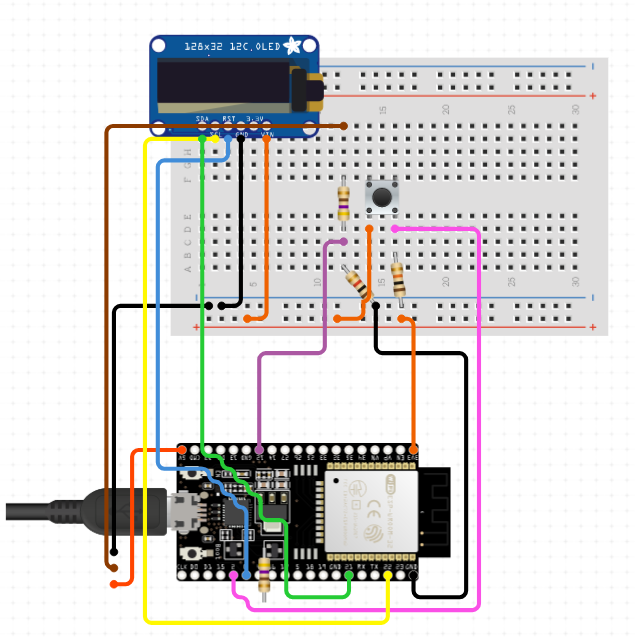
\includegraphics[width=0.75\textwidth]{imagenes/setup.png}
	\caption{Setup experimental}
\end{figure}
\subsection{Preparar ESP32 para Micropython}
Antes de poder usar el ESP32 para ejecutar python, debemos de grabar el firmware correspondiente a la placa. El proceso es bastante sencillo utilizando la herramienta Esptool\cite{ref17}:
\begin{itemize}
	\item En lugar de instalar la herramienta usando pip de python, recomiendo descargar el codigo fuente desde la pagina de github\cite{ref18} y ejecutar el archivo esptool.py directamente ya que al menos en mi experiencia da menos problemas.
	\item Una vez con la herramienta instalada, lo primero es borrar completamente la memoria flash de la placa. Ejecutaremos el siguiente comando(en mi caso, ttyUSB0 para indicar el puerto al que esta conectado):
\end{itemize}
\begin{lstlisting}[language=Bash]
	esptool.py --port /dev/ttyUSB0 erase_flash
\end{lstlisting}
\begin{itemize}
	\item Ahora, debemos de grabar el firmware de Micropython en la placa. Para ello, descargaremos el firmware (.bin) de la pagina oficial\cite{ref19} y ejecutaremos el siguiente comando:
\end{itemize}
\begin{lstlisting}[language=python]
	esptool.py --port /dev/ttyUSB0 write_flash -z 0x1000 esp32.bin
\end{lstlisting}
\begin{itemize}
	\item Si todo ha ido bien, ya podremos ejecutar Micropython en la placa. Podemos comprobarlo conectandonos por el puerto serie a la placa (en el ejemplo uso picocom pero se puede utilizar cualquier software que permita la conexion por serial) y viendo si la placa nos responde con el prompt de Micropython:
\end{itemize}
	\begin{lstlisting}
		$ picocom /dev/ttyUSB0 -b115200
	\end{lstlisting}
	\begin{figure}[h!]
		\centering
		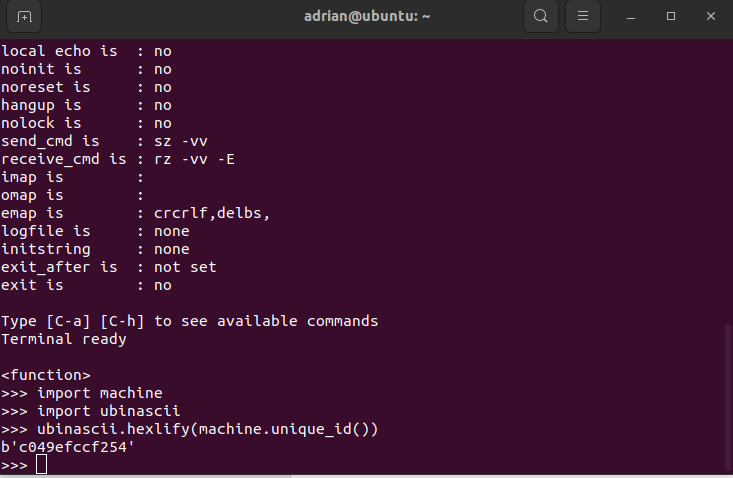
\includegraphics[width=0.75\textwidth]{imagenes/micropython_prompt.png}
		\caption{Prompt de Micropython}
	\end{figure}

\subsection{Micropython en ESP32}
Despues de instalar el firmware de Micropython en la placa, podremos observar que hay un archivo llamado boot.py que se ejecuta al arrancar la placa. En este archivo se puede configurar la placa para que se conecte a una red WiFi o para que se conecte a un servidor MQTT.\\
Despues de este boot.py, la placa intentará ejecutar el archivo main.py si existe. En este archivo se puede programar el comportamiento de la placa.\\

Al igual que en python, podemos hacer uso de diferentes librerias. Para poder usar librerias que no vengan por defecto en el firmware de Micropython, debemos de copiar los archivos .py a la flash de la placa con la herramienta Ampy de Adafruit\cite{ref20}. Con Ampy podemos desde copiar un archivo a la flash de la placa o recuperar un archivo de la flash de la placa a nuestro ordenador. \\
Uso de Ampy:
\begin{figure}[h!]
	\centering
	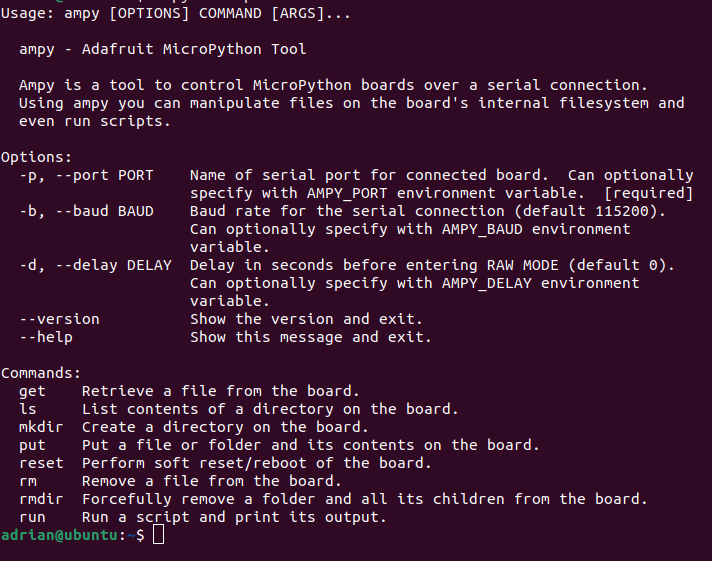
\includegraphics[width=0.75\textwidth]{imagenes/ampy.png}
	\caption{Opciones de Ampy}
\end{figure}
\subsection{Librerias utilizadas}
\subsubsection{Libreria para el SSD1306}
Para usar el modulo SSD1306, se ha utilizado la libreria \cite{ref21} en Micropython. Esta libreria nos permite inicializar el modulo SSD1306 y escribir texto en la pantalla de manera sencilla.\\
\subsubsection{Libreria para MQTT}
Para usar MQTT, se ha utilizado la libreria umqtt.simple\cite{ref22} en Micropython. Esta libreria nos permite conectarnos a un servidor MQTT y publicar y subscribirse a diferentes topics.\\
\newpage
\section{Implementación}
\subsection{Diagrama de estados}
\subsubsection{Init}
La inicialización del programa empieza por conectarse a la red WiFi y al broker de MQTT. A continuación comprobamos si ya hemos establecido conexión previamente con la aplicación web. Si no se ha establecido previamente conexión con la aplicación web, empezaremos a publicar periodicamente el ID interno del ESP32 y esperaremos a que la aplicaciób web nos devuelva el ACK. Lo siguiente es comprobar si hemos recibido la configuración de la aplicación web (la configuración a recibir es el tipo de sensor y el voltaje al que estamos conectados). Por último calibramos el sensor, es decir, leemos el voltaje de salida del ACS712 durante un periodo de tiempo sin que haya nada conectado al sensor y lo guardamos como voltaje de referencia para poder calcular la corriente en el futuro.\\
\begin{figure}[h!]
	\centering
	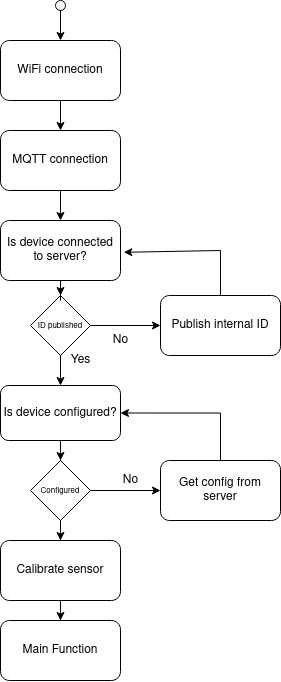
\includegraphics[width=0.30\textwidth]{imagenes/Init.drawio.png}
	\caption{Diagrama de estados Init}
\end{figure}
\subsubsection{Main}
La función principal es bastante sencilla. En cada iteración, lanzamos una llamada a la libreria de MQTT para comprobar si hay mensajes en la cola recibidos (esto hará que se lance el callback de recepción de mensajes MQTT si es que hay alguno). Si el sensor esta encendido, lo siguiente es leer el voltaje de salida del sensor de corriente y calcular el amperaje y consumo (en Watts). Estos watios calculados los mostramos por el dispositivo OLED que tenemos conectado. Por último, publicamos el valor del amperaje y consumo en el topic de MQTT correspondiente (watts/ID\_Sensor y amps/ID\_Sensor). En caso de que el sensor este apagado, no realizamos ninguna acción y esperamos a recibir el mensaje de encender por MQTT.\\


TODO: ACTUALIZAR DIAGRAMA DE ESTADOS CON LA CONDICION DE SENSING O NO SENSING

\begin{figure}[h!]
	\centering
	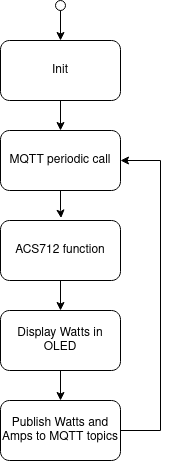
\includegraphics[width=0.30\textwidth]{imagenes/main.drawio.png}
	\caption{Diagrama de estados función Main}
\end{figure}
\newpage
\subsubsection{Lectura del sensor}
\begin{figure}[h!]
	\centering
	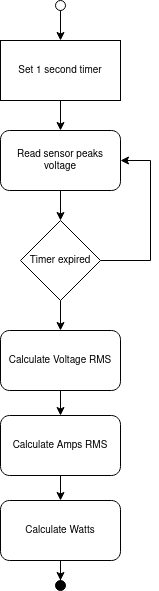
\includegraphics[width=0.30\textwidth]{imagenes/acs712.drawio.png}
	\caption{Diagrama de la función de lectura del ACS712}
\end{figure}

\subsection{Código}
\subsubsection{Función Init}
\begin{lstlisting}[language=python]
display_message('Connecting to WiFi...')
connect_wifi(SSID, PASSWORD)

#display_message('Connecting to MQTT broker...')
MQTT_CLIENT.connect()
MQTT_CLIENT.mqtt.set_callback(subscribe_callback)
if MQTT_CLIENT.is_broker_acknowledged() == False:
	MQTT_CLIENT.publish_clientID()

#Init value for relay is always on, i.e, after a reset we want the relay to be on
RELAY.value(1)
SENSING = True

#subscribe to reset topic
MQTT_CLIENT.subscribe('reset/' + MQTT_CLIENT.client_id.decode("utf-8"))
#subscribe to sensor_config topic to receive the sensor voltage
MQTT_CLIENT.subscribe('sensor_config/' + MQTT_CLIENT.client_id.decode("utf-8"))
#subscribe to relay topic to power on/off the devices
MQTT_CLIENT.subscribe('relay/' + MQTT_CLIENT.client_id.decode("utf-8"))

display_message('Configuring sensor...')
if CURRENT_SENSOR.is_sensor_configured() == False or VOLTAGE_SENSOR.is_sensor_configured() == False:
	MQTT_CLIENT.get_sensor_config_from_broker()

#subscribe to restart esp32 topic
MQTT_CLIENT.subscribe('restart/' + MQTT_CLIENT.client_id.decode("utf-8"))

display_message('Calibrating amp sensor...')
CURRENT_SENSOR.calibrateSensorAC(RELAY)

display_message('Calibrating voltage sensor...')
VOLTAGE_SENSOR.calibration(RELAY)


#subscribe to calibrate topic
MQTT_CLIENT.subscribe('calibrate/' + MQTT_CLIENT.client_id.decode("utf-8"))
\end{lstlisting}

\subsubsection{Función de calibración del sensor de corriente ACS712}
\begin{lstlisting}[language=python]
def calibrateSensorAC(self, seconds=10):
	"""
	Calibrate the sensor to get the average voltage 
	reading when there is no load.
	"""
	print("[testCalibrateSensor]Calibrating sensor...")
	print("[testCalibrateSensor]Please disconnect the sensor \
		from the load NOW!")
	for i in reversed(range(5)):
		print("[testCalibrateSensor]Starting calibration in " + 
			str(i+1) + " seconds...")
		utime.sleep(0.5)
	print("[testCalibrateSensor]Calibrating...")
	counter = 0
	voltage_RMS = 0
	average_voltage = 0
	start = time.ticks_ms()
	while time.ticks_ms() - start < (1000 * seconds):
		min_value = 4095
		max_value = 0
		voltage = 0
		for i in range(100):
			adc_raw = self.adc.read()
			voltage += adc_raw
			if adc_raw < min_value:
				min_value = adc_raw
			elif adc_raw > max_value:
				max_value = adc_raw
			time.sleep_us(500)
		average_voltage += ((voltage * 3.3) / 4095) / 100
		counter = counter + 1
		max_value_V = ((max_value * 3.3) / 4095)
		min_value_V = ((min_value * 3.3) / 4095)
		peak_to_peak = (max_value_V - min_value_V)
		voltage_RMS += peak_to_peak * 0.3536
	end = time.ticks_ms()
	print("[readAmps2]Time to read ", counter, " values: ", 
		time.ticks_diff(end, start), "ms")
	voltage_RMS = voltage_RMS / counter
	if voltage_RMS > 0.020:
		self.default_VRMS = voltage_RMS
	else:
		self.default_VRMS = 0.020
	self.default_output_voltage = average_voltage / counter
	#add 5mV to the default output voltage to avoid negative values
	self.default_VRMS = self.default_VRMS + 0.005
	print("[calibrateSensorAC]Sensor calibrated. Default output \
			voltage: ", self.default_output_voltage, "V")
	print("[calibrateSensorAC]Sensor calibrated. Default VRMS: ", 
			self.default_VRMS, "V")
\end{lstlisting}

\subsubsection{Función Main}
\begin{lstlisting}[language=python]
init()

while True:
	MQTT_CLIENT.check_msg()
	if SENSING == True:
		voltage = VOLTAGE_SENSOR.getVoltage()
		watts, amps = CURRENT_SENSOR.getACWatts(voltage_from_sensor=voltage, logging=False)
		display_watts(watts)
		MQTT_CLIENT.publish('voltage/' + MQTT_CLIENT.client_id.decode("utf-8"), str(voltage))
		MQTT_CLIENT.publish('amps/' + MQTT_CLIENT.client_id.decode("utf-8"), str(amps))
		MQTT_CLIENT.publish('watts/' + MQTT_CLIENT.client_id.decode("utf-8"), str(watts))
		print('-----------------------')
	else:
		print("Sensing is disabled")
		utime.sleep(1)
\end{lstlisting}

\subsubsection{Funciones de lectura del sensor de corriente}
\begin{lstlisting}[language=python]
def readSensorVPP(self, logging=False):
	"""
	Capture the peak to peak voltage of the current ADC signal.
	Period of measurement is 50ms. The ADC is sampled every 500us. 
	100 samples are taken. AC current in spain is 50Hz.
	We should be able to capture at least 2 full cycles of the 
	sinusoidal signal with its peaks.
	"""
	min_value = 4095
	max_value = 0
	average_value = 0
	start = time.ticks_ms()
	for i in range(100):
		adc_raw = self.adc.read()
		average_value += adc_raw
		if adc_raw < min_value:
			min_value = adc_raw
		elif adc_raw > max_value:
			max_value = adc_raw
		time.sleep_us(500)
	end = time.ticks_ms()
	max_value_V = ((max_value * 3.3) / 4095)
	min_value_V = ((min_value * 3.3) / 4095)
	average_value_V = ((average_value / 100) * 3.3) / 4095
	peak_to_peak = (max_value_V - min_value_V)
	if logging:
		print("[readSensorVPP]Time to read 100 samples: ", 
				time.ticks_diff(end, start), "ms")
		print("[readSensorVPP]Average value: ", average_value_V, "V")
		print("[readSensorVPP]Max value: ", max_value_V, "V; Min \
			value: ", min_value_V, "V; VPP: ", peak_to_peak, "V")

	return peak_to_peak, average_value_V 

def readRMSVoltage(self, logging=False):
	voltage_RMS = 0
	voltage_RMS_nofilter = 0
	average_voltage = 0
	samplesVPP = list()
	samplesV = list()
	start = time.ticks_ms()
	while time.ticks_ms() - start < 1000:
		voltagePP, voltage = self.readSensorVPP(logging=False)
		samplesVPP.append(voltagePP * 0.3536)
		samplesV.append(voltage)
	end = time.ticks_ms()
	for i in range(len(samplesVPP)):
		voltage_RMS_nofilter += samplesVPP[i]
		average_voltage += samplesV[i]
	"""
	for sample in samplesVPP:
		voltage_RMS_nofilter += sample
	"""
	voltage_RMS_nofilter = voltage_RMS_nofilter / len(samplesVPP)
	average_voltage = average_voltage / len(samplesV)
	#apply sw filter
	samplesVPP = self.RMSFilter(samplesVPP, logging=False)
	for sample in samplesVPP:
		voltage_RMS += sample
	voltage_RMS = voltage_RMS / len(samplesVPP)

	if logging:
		print("[readRMSVoltage]Time to read ", len(samplesV), 
			" values: ", time.ticks_diff(end, start), "ms")
		print("[readRMSVoltage]Voltage RMS: ", voltage_RMS * 1000, 
			"mV", " default VRMS: ", self.default_VRMS * 1000, "mV")
		print("[readRMSVoltage]Voltage RMS no filter: ", 
			voltage_RMS_nofilter * 1000, "mV", " default VRMS: ", 
				self.default_VRMS * 1000, "mV")
		print("[readRMSVoltage]Average voltage: ", 
			average_voltage * 1000, "mV"," default output voltage: ", 
				self.default_output_voltage * 1000, "mV")
	
	return voltage_RMS, average_voltage

def readRMSAmps(self, logging=False):
	voltage_RMS, voltage = self.readRMSVoltage(logging=logging)
	#decide whether to apply an error correction or not
	if self.checkZeroRange(voltage_RMS, voltage, logging=logging):
		Amps_RMS = 0
	else:
		Amps_RMS = (voltage_RMS * 1000) / self.scale_factor

	amps = abs(((voltage - self.default_output_voltage) * 1000)
		 / self.scale_factor)
	if logging:
		print("[readRMSAmps]Current: ", Amps_RMS, "A RMS")
		print("[readRMSAmps]Current: ", amps, "A")

	return Amps_RMS, amps

def getACWatts(self, logging=False):
	"""
	Calculate the power consumption in Watts.
	"""
	Amps_RMS, amps = self.readRMSAmps(logging=logging)
	if self.type == "AC":
		watts = self.referenceVoltage * Amps_RMS
		ret_amps = Amps_RMS
	elif self.type  == "DC":
		watts = self.referenceVoltage * amps
		ret_amps = amps
	else:
		watts = 0
	if logging:
		print("[getACWatts]Watts: ", watts, "W", "with sensor: ", 
				self.type)

	return watts, ret_amps

\end{lstlisting}

El codigo completo puede ser consultado en el siguiente enlace\cite{ref23}.\\


\section {Voltaje variable}
\subsection{Problema}
Hasta ahora, como se ha podido ver, teniamos los valores de voltaje hardcodeados en el código. Esto no es una buena práctica, ya que si queremos cambiar el voltaje de referencia, tendremos que modificar el código aunque hayamos comtemplado los valores estandares en Europa: 210, 220 y 230 voltios para corriente alterna y 12, 24 y 48 para corriente continua. Tal y como tenemos este proyecto, sin modificar el codigo no podriamos usarlo en paises donde la corriente alterna sea de 110 voltios por ejemplo. Por lo tanto, se ha decidido implementar un sensor de voltaje que nos permita leer el voltaje de la red y asi poder usar el valor del voltaje en tiempo real para calcular el consumo de energia.\\

\subsection{Sensor de voltaje}
Se ha decidido usar el sensor ZMPT101B que es capaz de leer voltajes de 0 a 1000V. Este sensor tiene una salida de 0 a 5V, por lo que no se puede conectar directamente a la entrada analógica del ESP32. Para poder usarlo, se ha usado un divisor de tensión de la misma forma que lo hicimos para el sensor de corriente y asi obtener la señal en un rango de 0 a 3.3V.\\

INSERTAR IMAGEN DEL SENSOR\\

Para obtener el valor del voltaje, haremos uso de una ecuación lineal tomando como puntos de referencia el valor del sensor sin ningun voltaje aplicado y el valor del sensor con un voltaje dado durante la calibración de este (el valor lo obtendremos usando un multimetro y midiendo el voltaje de la red). La ecuación lineal es la siguiente: \\
\begin{equation}
	V_{out} = \frac{V_{in} - V_{in,0}}{V_{in,1} - V_{in,0}} \cdot (V_{out,1} - V_{out,0}) + V_{out,0}
\end{equation}
Donde $V_{in}$ es el valor de entrada del sensor, $V_{in,0}$ es el valor de entrada del sensor sin ningun voltaje aplicado, $V_{in,1}$ es el valor de entrada del sensor con un voltaje dado durante la calibración de este, $V_{out}$ es el valor de salida del sensor, $V_{out,0}$ es el valor de salida del sensor sin ningun voltaje aplicado y $V_{out,1}$ es el valor de salida del sensor con un voltaje dado durante la calibración de este.\\

\subsection{Actualización del circuito}
INSERTAR IMAGEN DEL CIRCUITO CON EL NUEVO SENSOR

\subsection{Código}
\begin{lstlisting}[language=python]
	import machine
	import time
	import os
	
	class ZMPT101B:
		def __init__(self, pin):
			self.pin = machine.Pin(pin, machine.Pin.IN)
			self.adc = machine.ADC(self.pin)
			self.adc.atten(machine.ADC.ATTN_11DB)
			self.ac_voltage = 0
			self.no_load_voltage = 0
			self.load_voltage = 0
	
		def set_sensor_config(self, voltage):
			self.ac_voltage = float(voltage)
	
		def is_sensor_configured(self):
			for file in os.listdir():
				if file == 'sensor_configured.cfg':
					with open('sensor_configured.cfg', 'r') as file:
						stored_value = file.read()
						try: 
							_, sensor_voltage, _ = stored_value.split(',')
							if float(sensor_voltage) > 0:
								self.ac_voltage = float(sensor_voltage)
								print("[is_sensor_configured]Voltage sensor max voltage set to ", self.load_voltage)
								return True
						except ValueError:
							print("[is_sensor_configured]Invalid sensor config stored in flash")
							self.ac_voltage = 0
							return False
					break #file found, no need to continue
	
			return False #file not found or config invalid
	
		def getVPP(self):
			"""
			Capture the peak to peak voltage of the current ADC signal.
			Period of measurement is 50ms. The ADC is sampled every 500us. 100 samples are taken.
			AC current in spain is 50Hz.
			We should be able to capture at least 2 full cycles of the sinusoidal signal with its peaks.
			"""
			min_value = 4095
			max_value = 0
			average_value = 0
			for i in range(100):
				adc_raw = self.adc.read()
				average_value += adc_raw
				if adc_raw < min_value:
					min_value = adc_raw
				elif adc_raw > max_value:
					max_value = adc_raw
				time.sleep_us(500)
			max_value_V = ((max_value * 3.3) / 4095)
			min_value_V = ((min_value * 3.3) / 4095)
	
			return max_value_V, min_value_V
	
	
		def calibration(self, relay, calibration_time=10, input_from_user=False):
			#first read voltage without load, so turn off relay
			print("[calibration]Calibrating voltage sensor...")
			print("[calibration]Turning off relay")
			relay.value(0)
			#during calibration_time, get average of max and min value from adc
			values = []
			start = time.ticks_ms()
			while time.ticks_ms() - start < (calibration_time/2) * 1000:
				max, min = self.getVPP()
				values.append((max - min) * 0.3536)
			end = time.ticks_ms()
			
			self.no_load_voltage = sum(values) / len(values)
	
			print("[calibration]No load voltage: " + str(self.no_load_voltage) + "V in " + str(end - start) + "ms")
			
			print("[calibration]Turning on relay")
			#now, read voltage with load and get input from user
			relay.value(1)
			values_load = []
			start = time.ticks_ms()
			while time.ticks_ms() - start < (calibration_time/2) * 1000:
				max, min = self.getVPP()
				values_load.append((max - min) * 0.3536)
			end = time.ticks_ms()
			
			self.load_voltage = sum(values_load) / len(values_load)
			print("[calibration]Load voltage: " + str(self.load_voltage) + "V in " + str(end - start) + "ms")
			if input_from_user:
				ac_voltage = input("AC voltage measured with multimeter: ")
				self.ac_voltage = float(ac_voltage)
				print("[calibration]AC voltage set to " + str(self.ac_voltage) + "V")
			else:
				print("[calibration]AC voltage received from app " + str(self.ac_voltage) + "V")
		
		def getVoltage(self):
			"""
			Use linear equation to get voltage. x1, y1, x2, y2 are the points used to calculate the equation.
			"""
			x1 = self.no_load_voltage
			y1 = 0
			x2 = self.load_voltage
			y2 = self.ac_voltage
			m = (y2 - y1) / (x2 - x1)
			b = y1 - m * x1
	
			values_load = []
			start = time.ticks_ms()
			while time.ticks_ms() - start < 1000:
				max, min = self.getVPP()
				values_load.append((max - min) * 0.3536)
			voltage = sum(values_load) / len(values_load)
			ac_voltage = m * voltage + b
	
			return ac_voltage
\end{lstlisting}

\section{Test de funcionamiento}
\subsection{Corriente continua}
Para probar diferente amperajes se ha utilizado una fuente de alimentación que permite variar la corriente de salida entre 0 y 3A. La tensión de la fuente se ha fijado en 12V.\\
\subsubsection{No load}
\begin{figure}[h!]
	\centering
	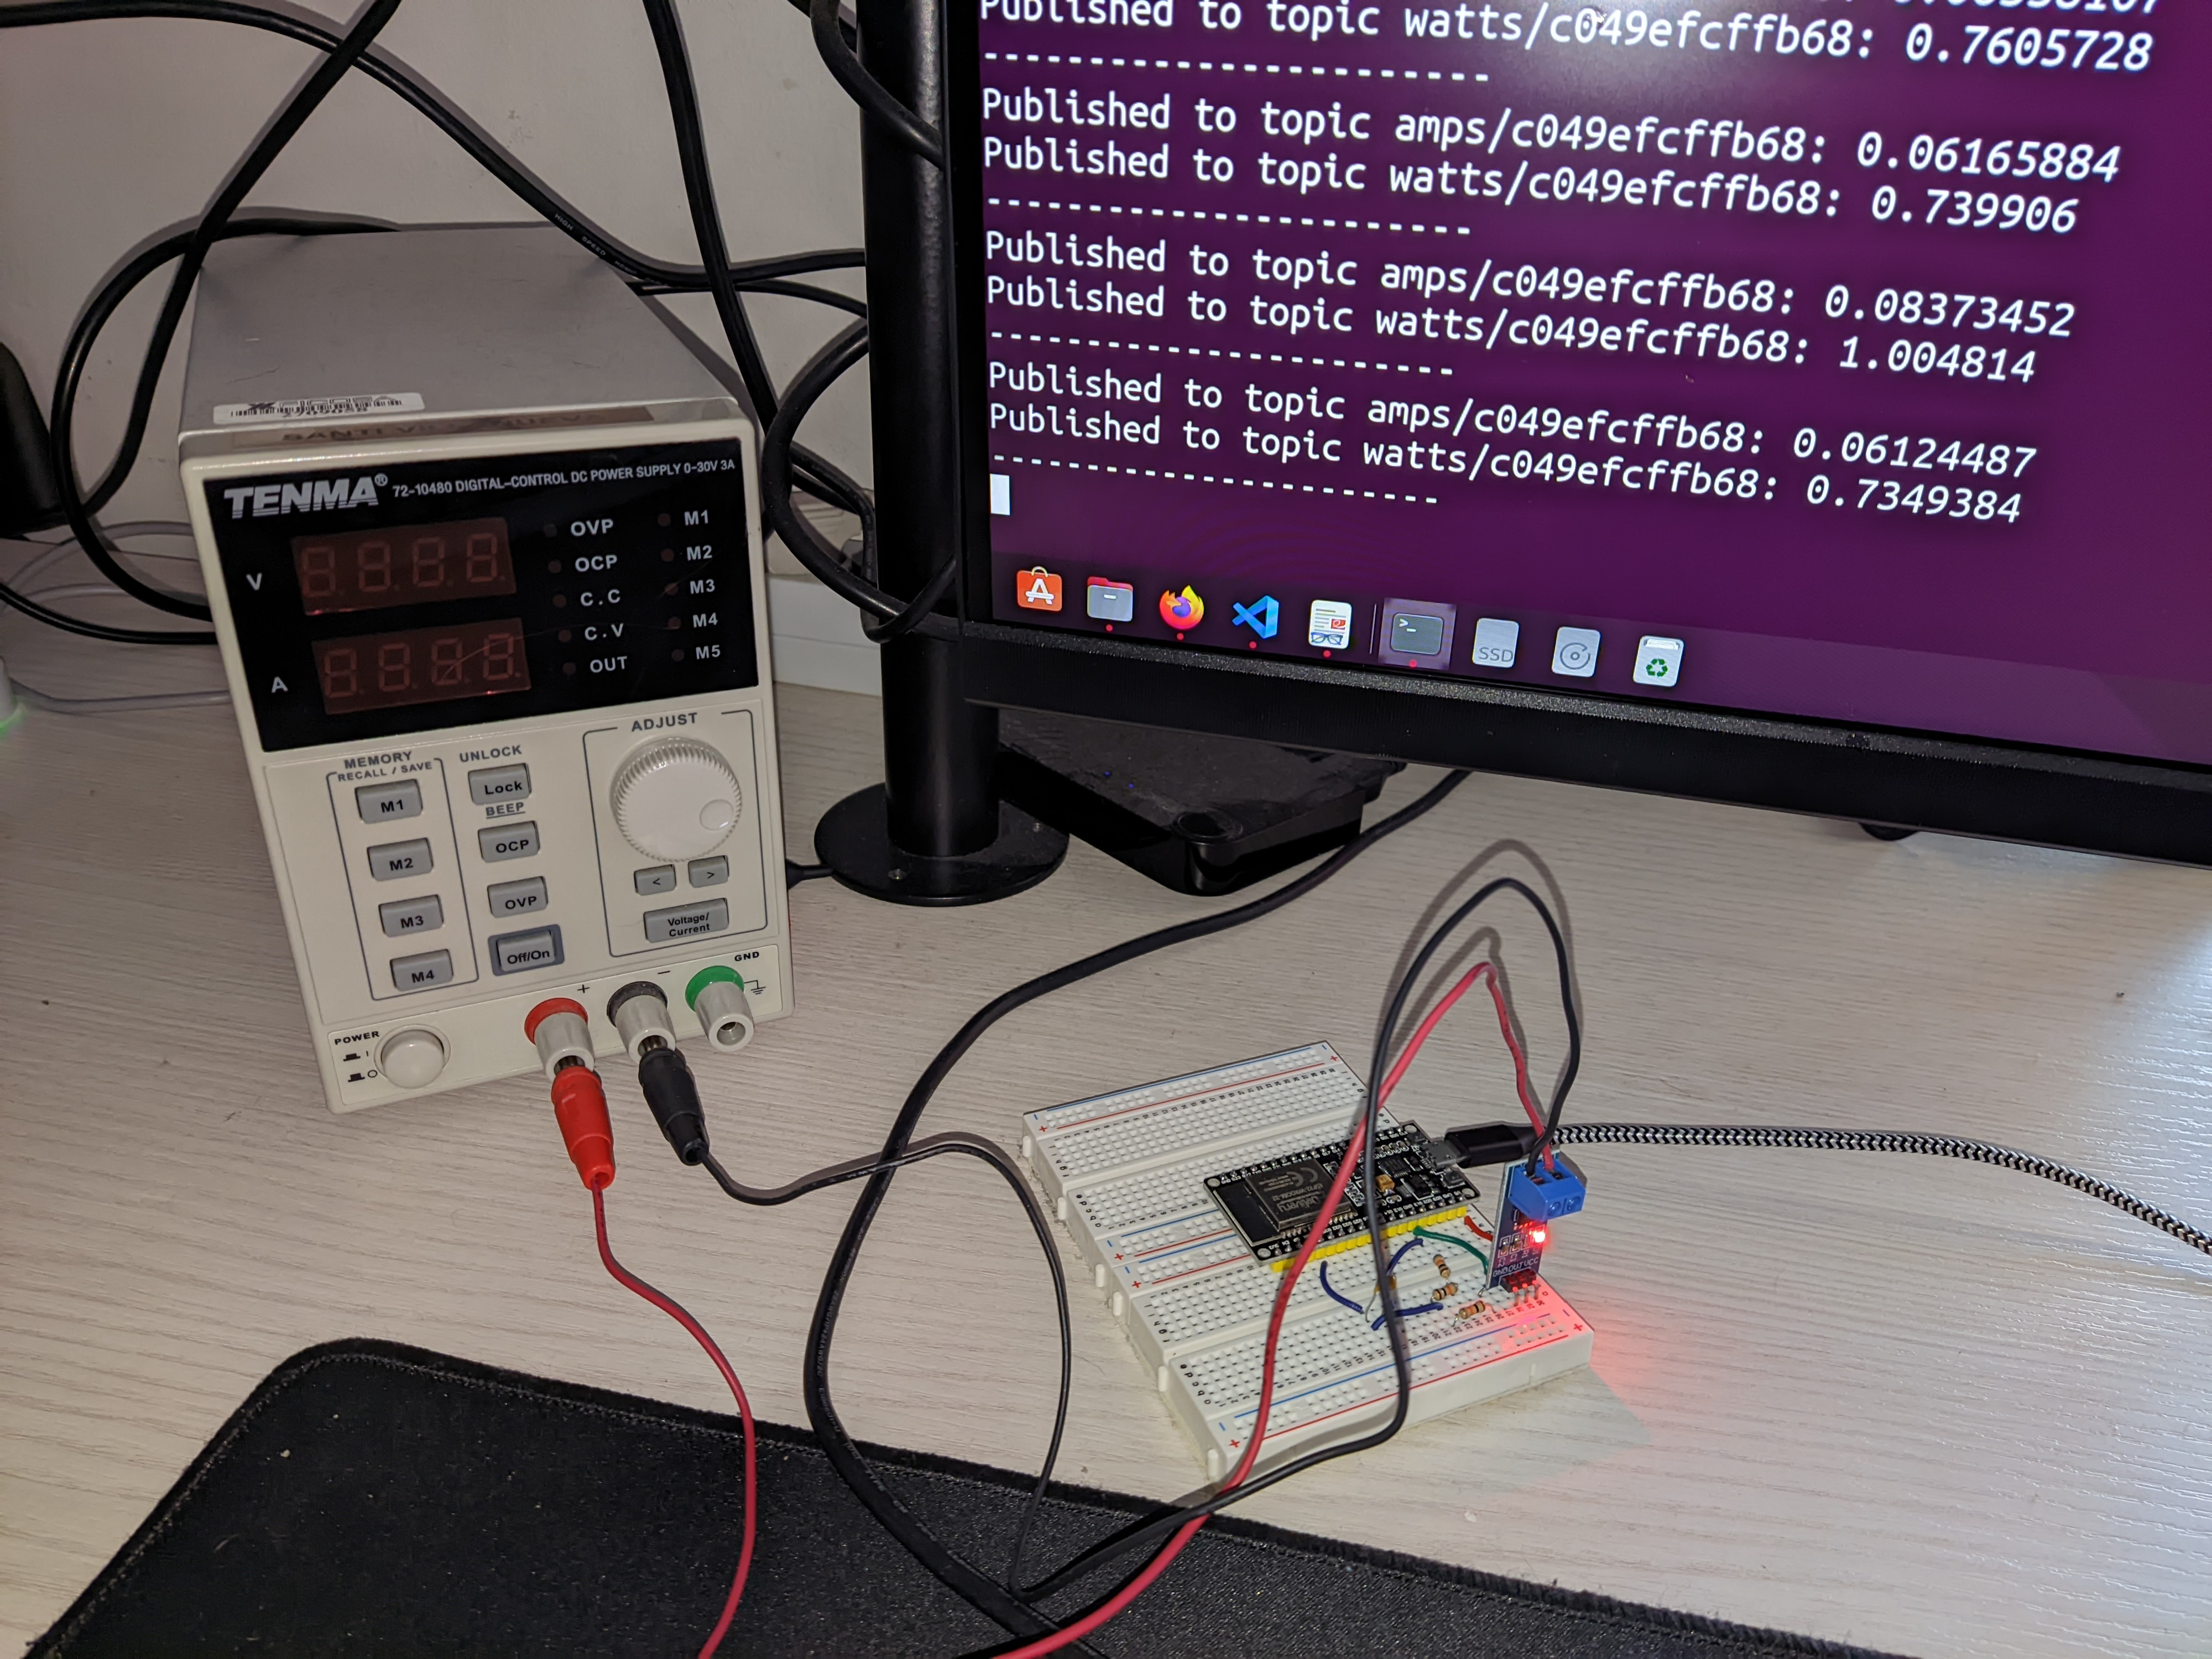
\includegraphics[width=0.5\textwidth]{imagenes/DC_noload.jpg}
	\caption{Salida del ACS712 con corriente continua de 0A}
\end{figure}
Como podemos observar, tras la conversión de la señal del ACS712 a amperios, tenemos valores muy cercanos a 0A que son practicamente despreciables. \\
\subsubsection{1A}
\begin{figure}[h!]
	\centering
	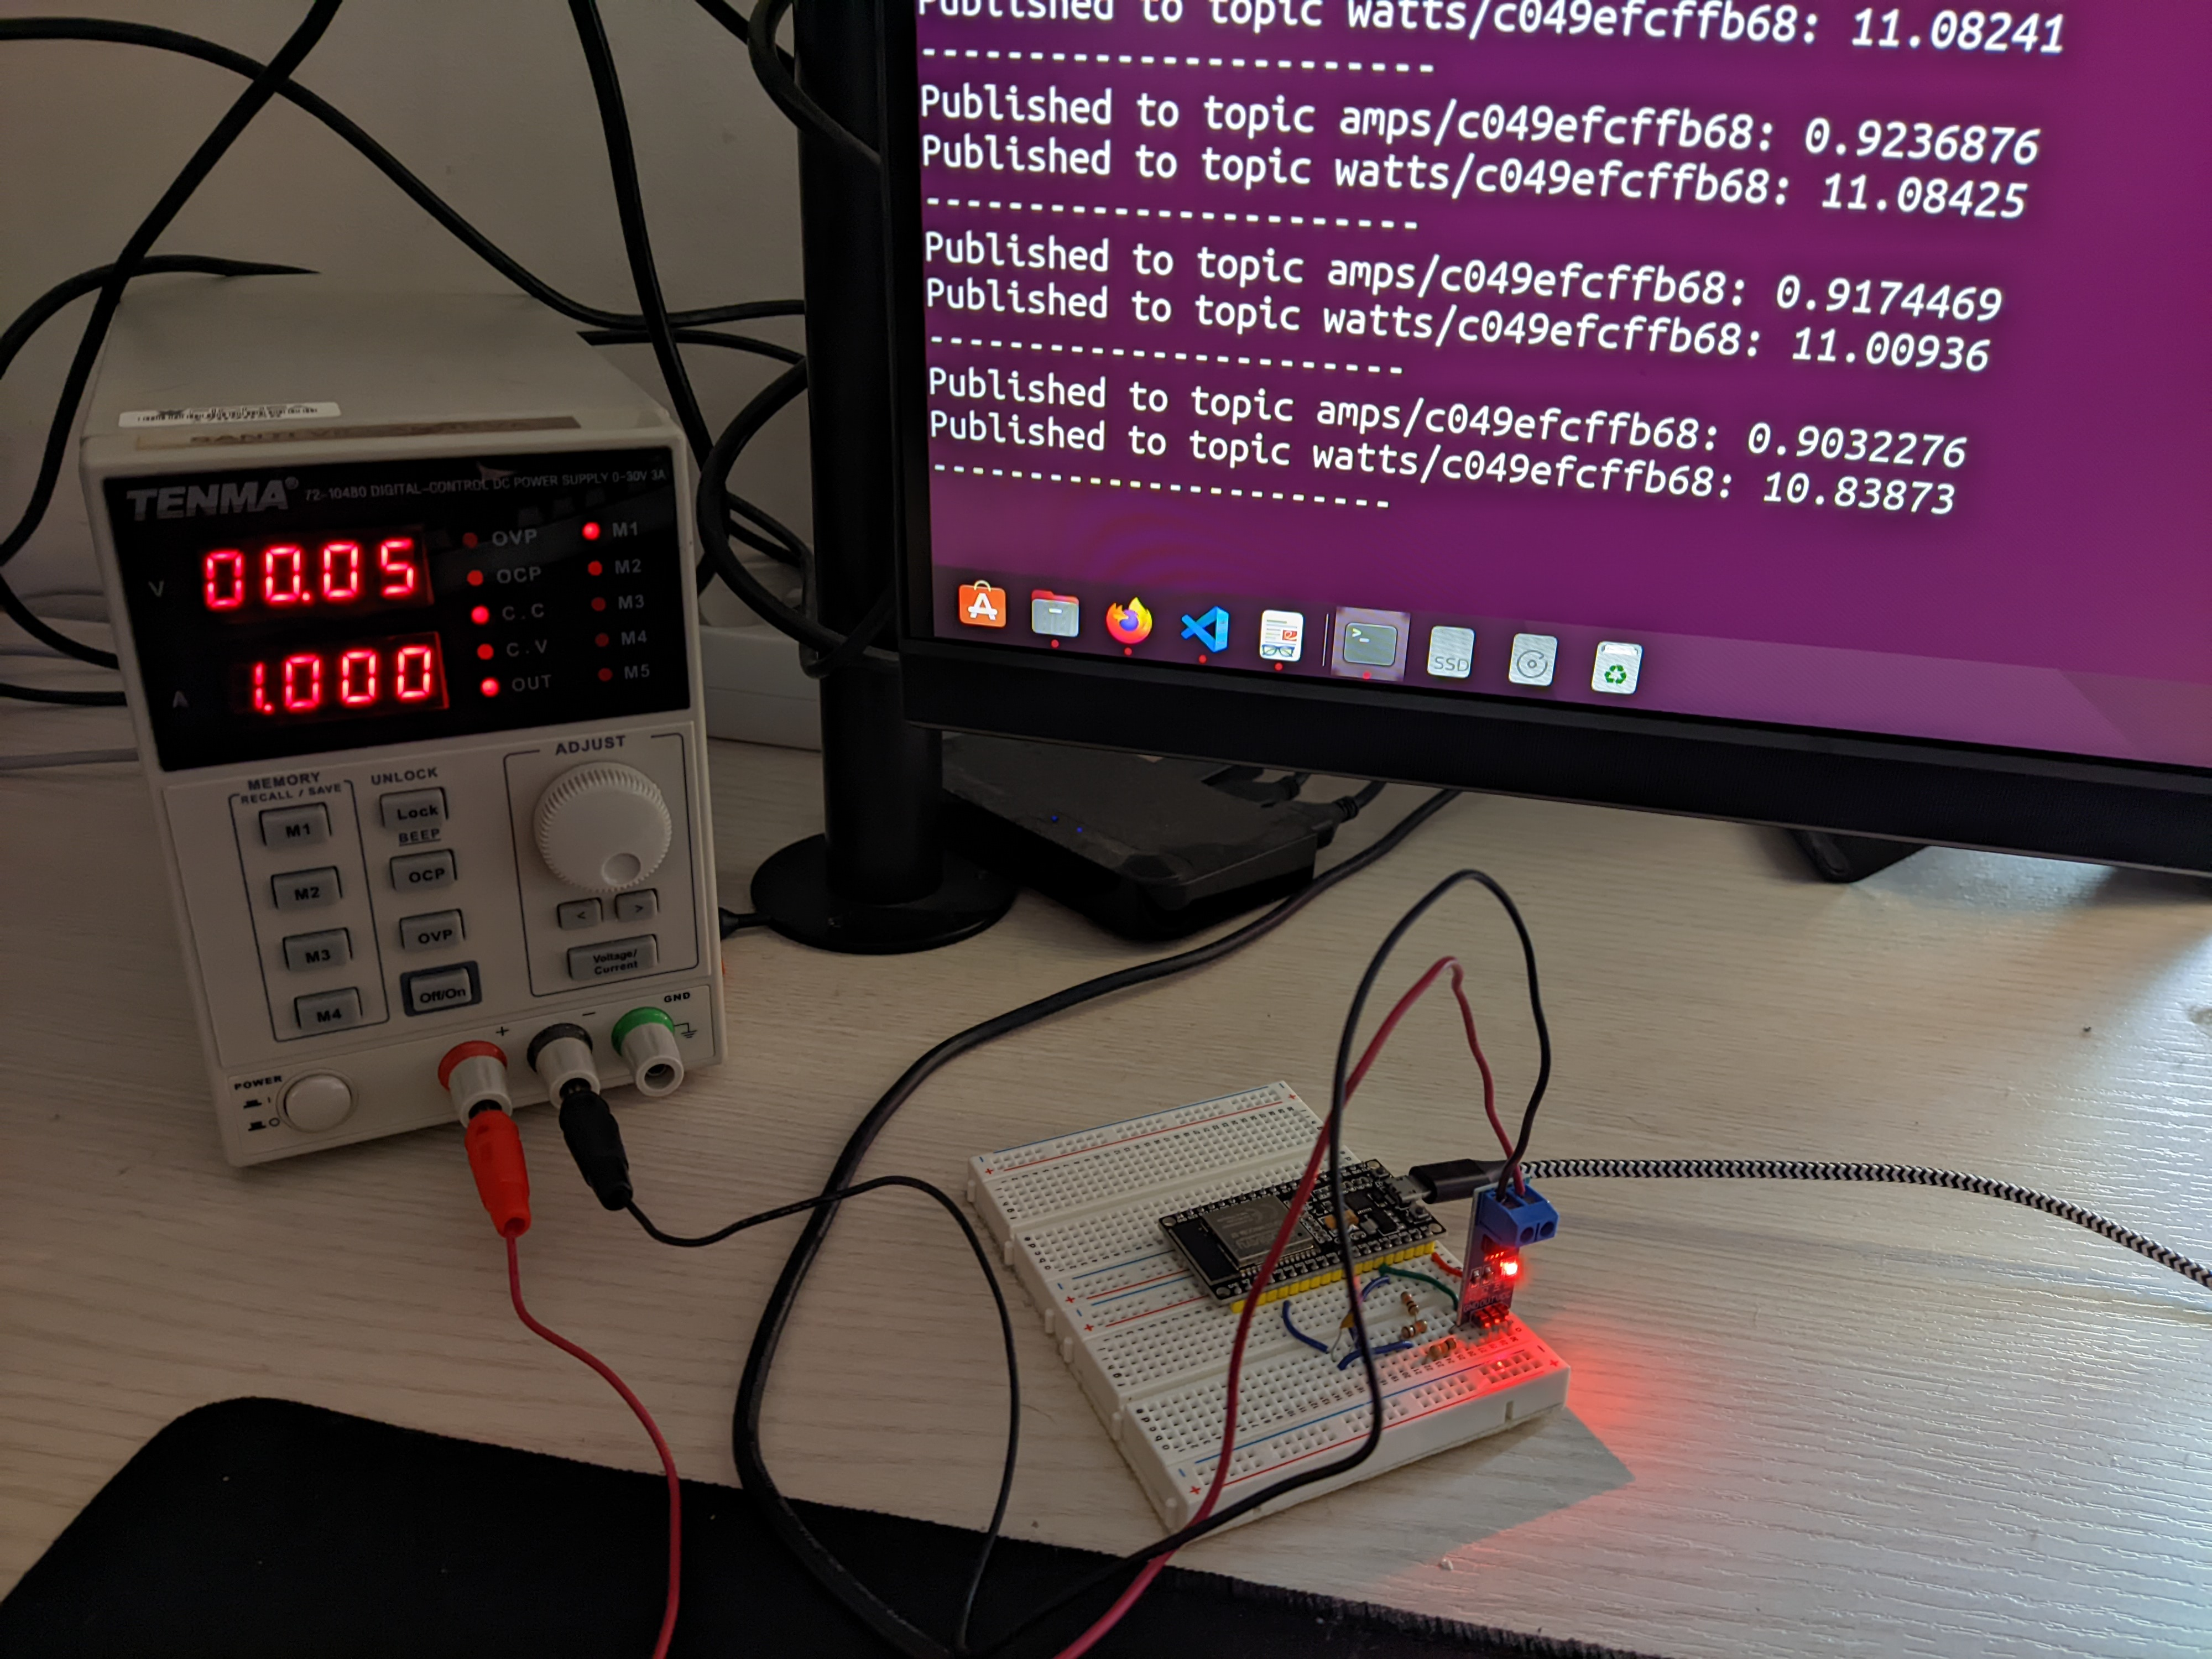
\includegraphics[width=0.5\textwidth]{imagenes/DC_1Amp.jpg}
	\caption{Salida del ACS712 con corriente continua de 1A}
\end{figure}
Generando 1A de corriente continua, medimos 0.91A con el sensor ACS712. \\
\subsubsection{1.7A}
\begin{figure}[h!]
	\centering
	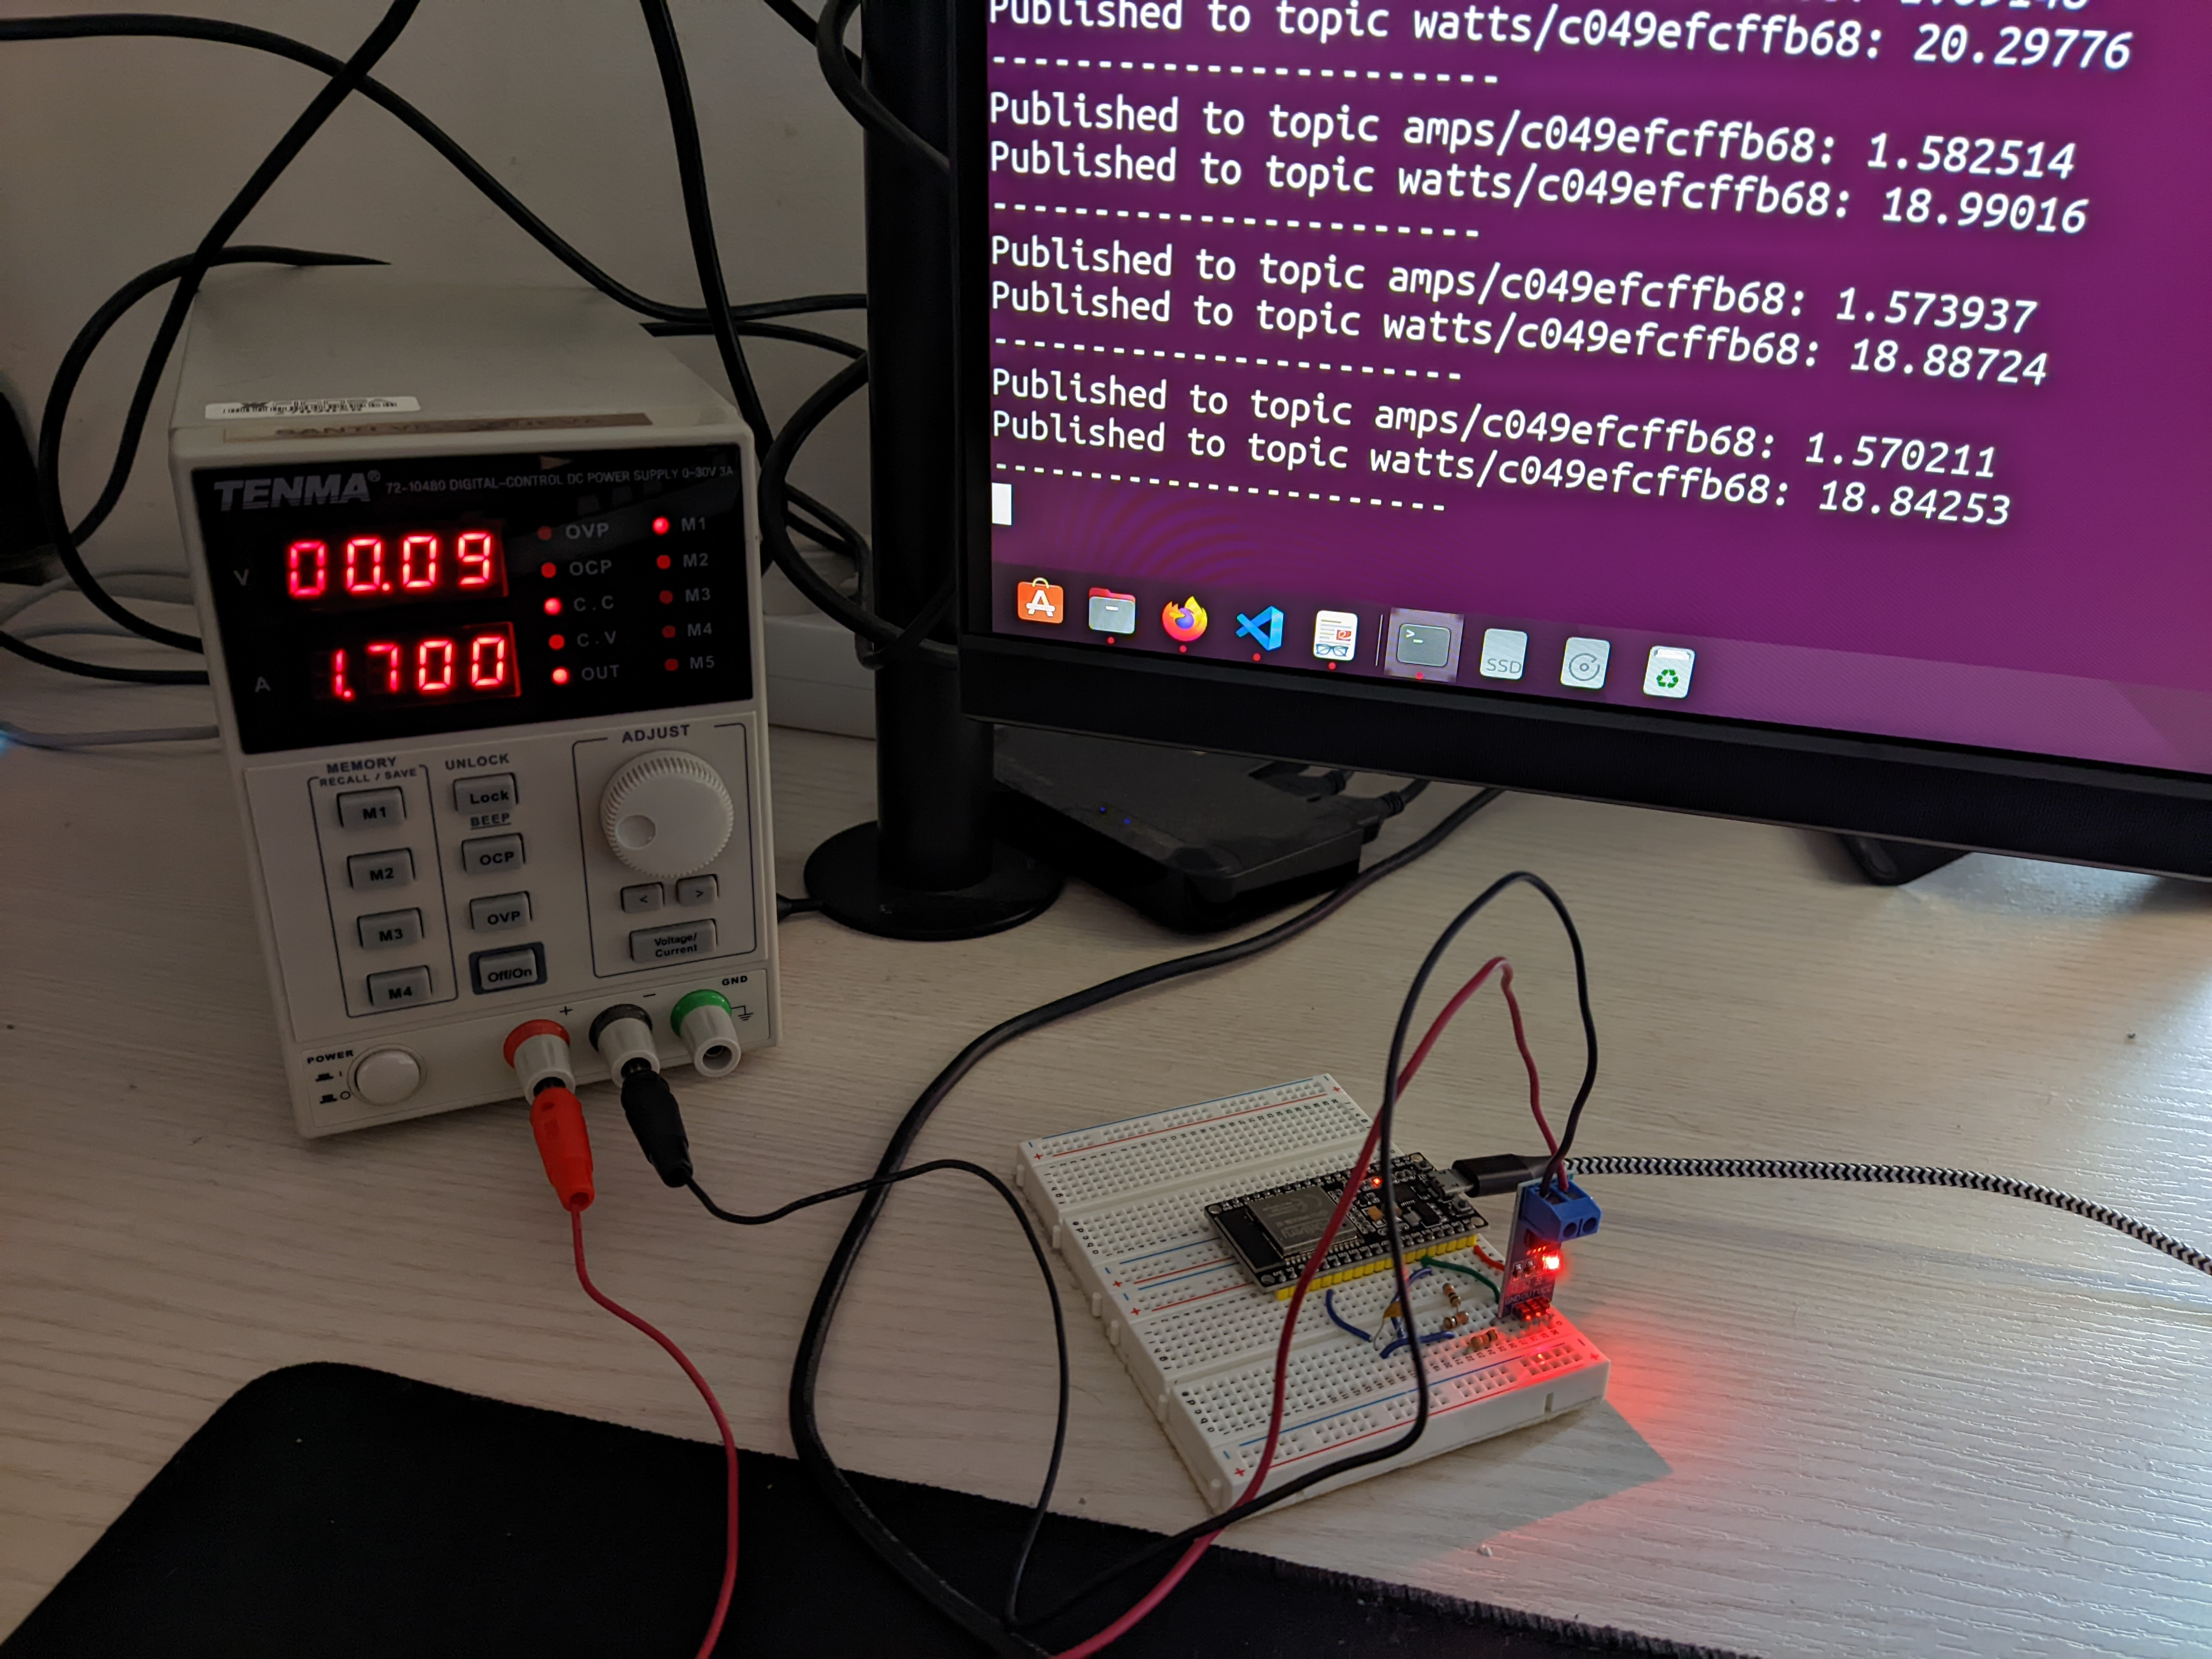
\includegraphics[width=0.5\textwidth]{imagenes/DC_1_7Amp.jpg}
	\caption{Salida del ACS712 con corriente continua de 1.7A}
\end{figure}
Generando 1.7A de corriente continua, medimos 1.58A con el sensor ACS712. \\
\subsubsection{3A}
\begin{figure}[h!]
	\centering
	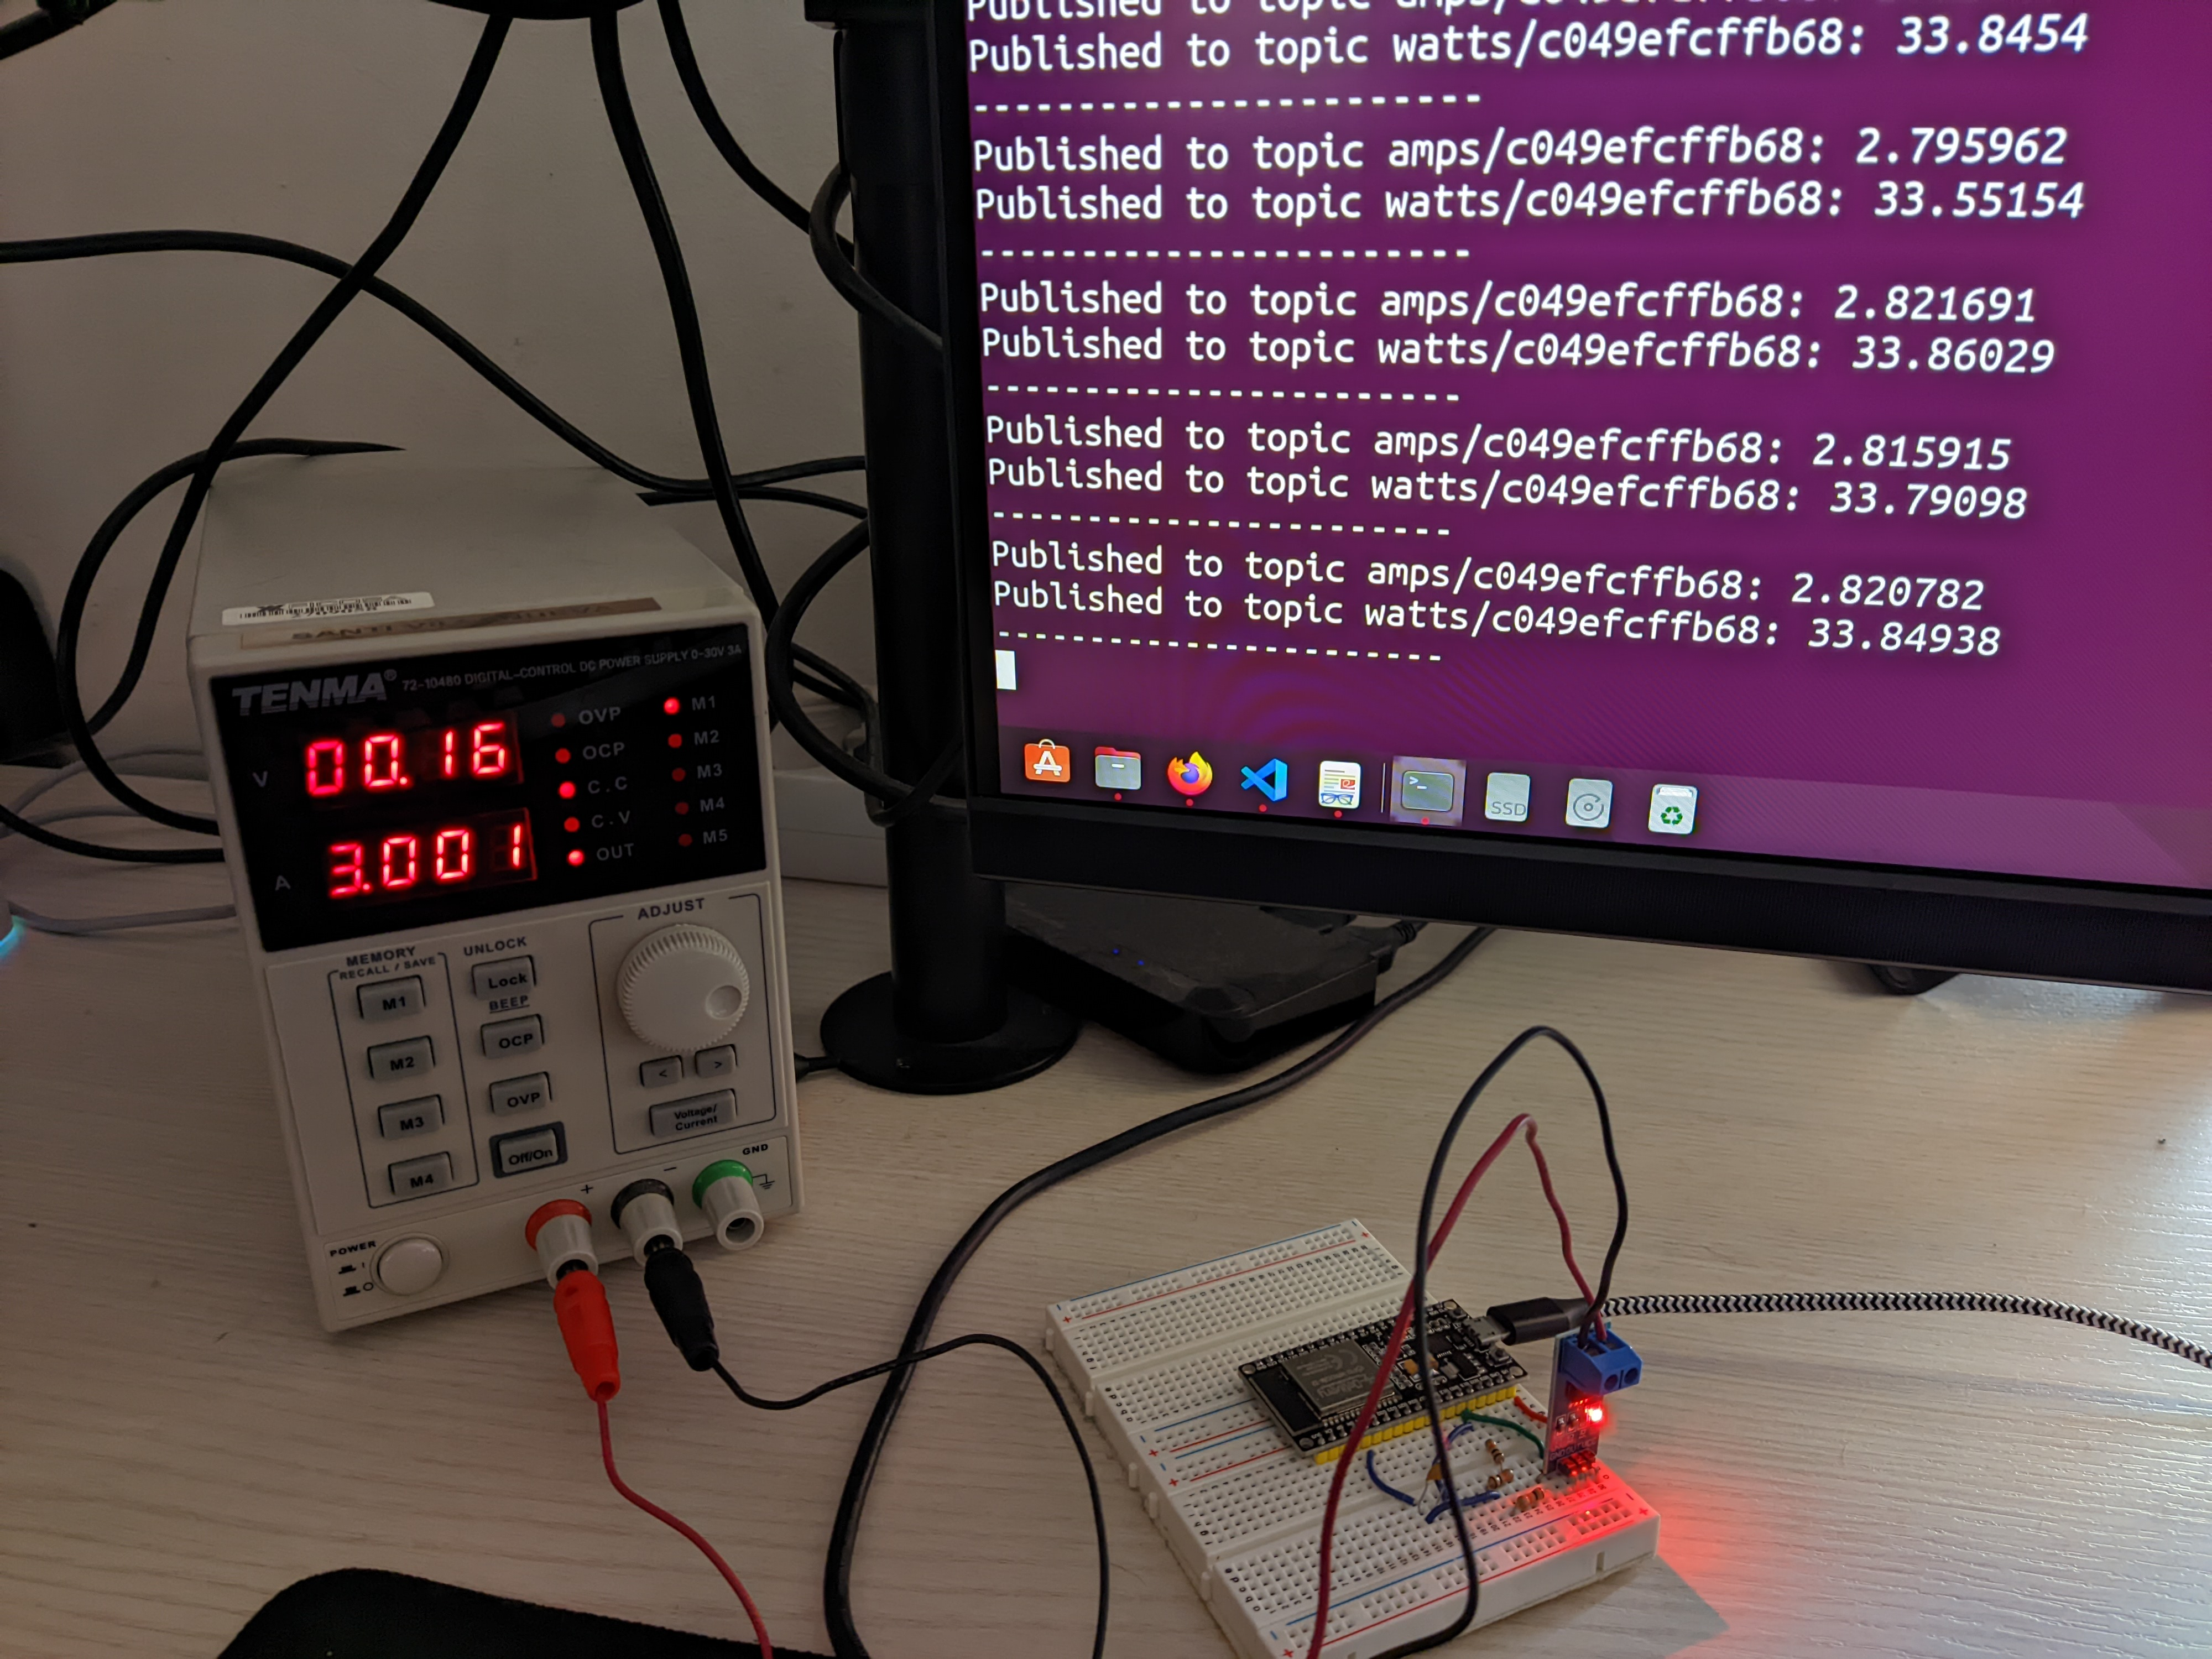
\includegraphics[width=0.5\textwidth]{imagenes/DC_3Amps.jpg}
	\caption{Salida del ACS712 con corriente continua de 3A}
\end{figure}
Generando 3A de corriente continua, medimos 2.82A con el sensor ACS712. \\

\subsection{Corriente alterna}
Como no dispongo de un generador de corriente alterna, he utilizado diferentes aparatos electricos para poder medir el consumo y el resultado del ACS712 se ha comparado con un amperimetro. El ACS712 esta conectado midiendo la corriente que pasa por el cable de una regleta de enchufes.\\
\subsubsection{No load}
Para la prueba de no tener ningun dispositivo conectado, simplemente se ha medido sin tener ningun enchufe conectado a la regleta.\\
\begin{figure}[h!]
	\centering
	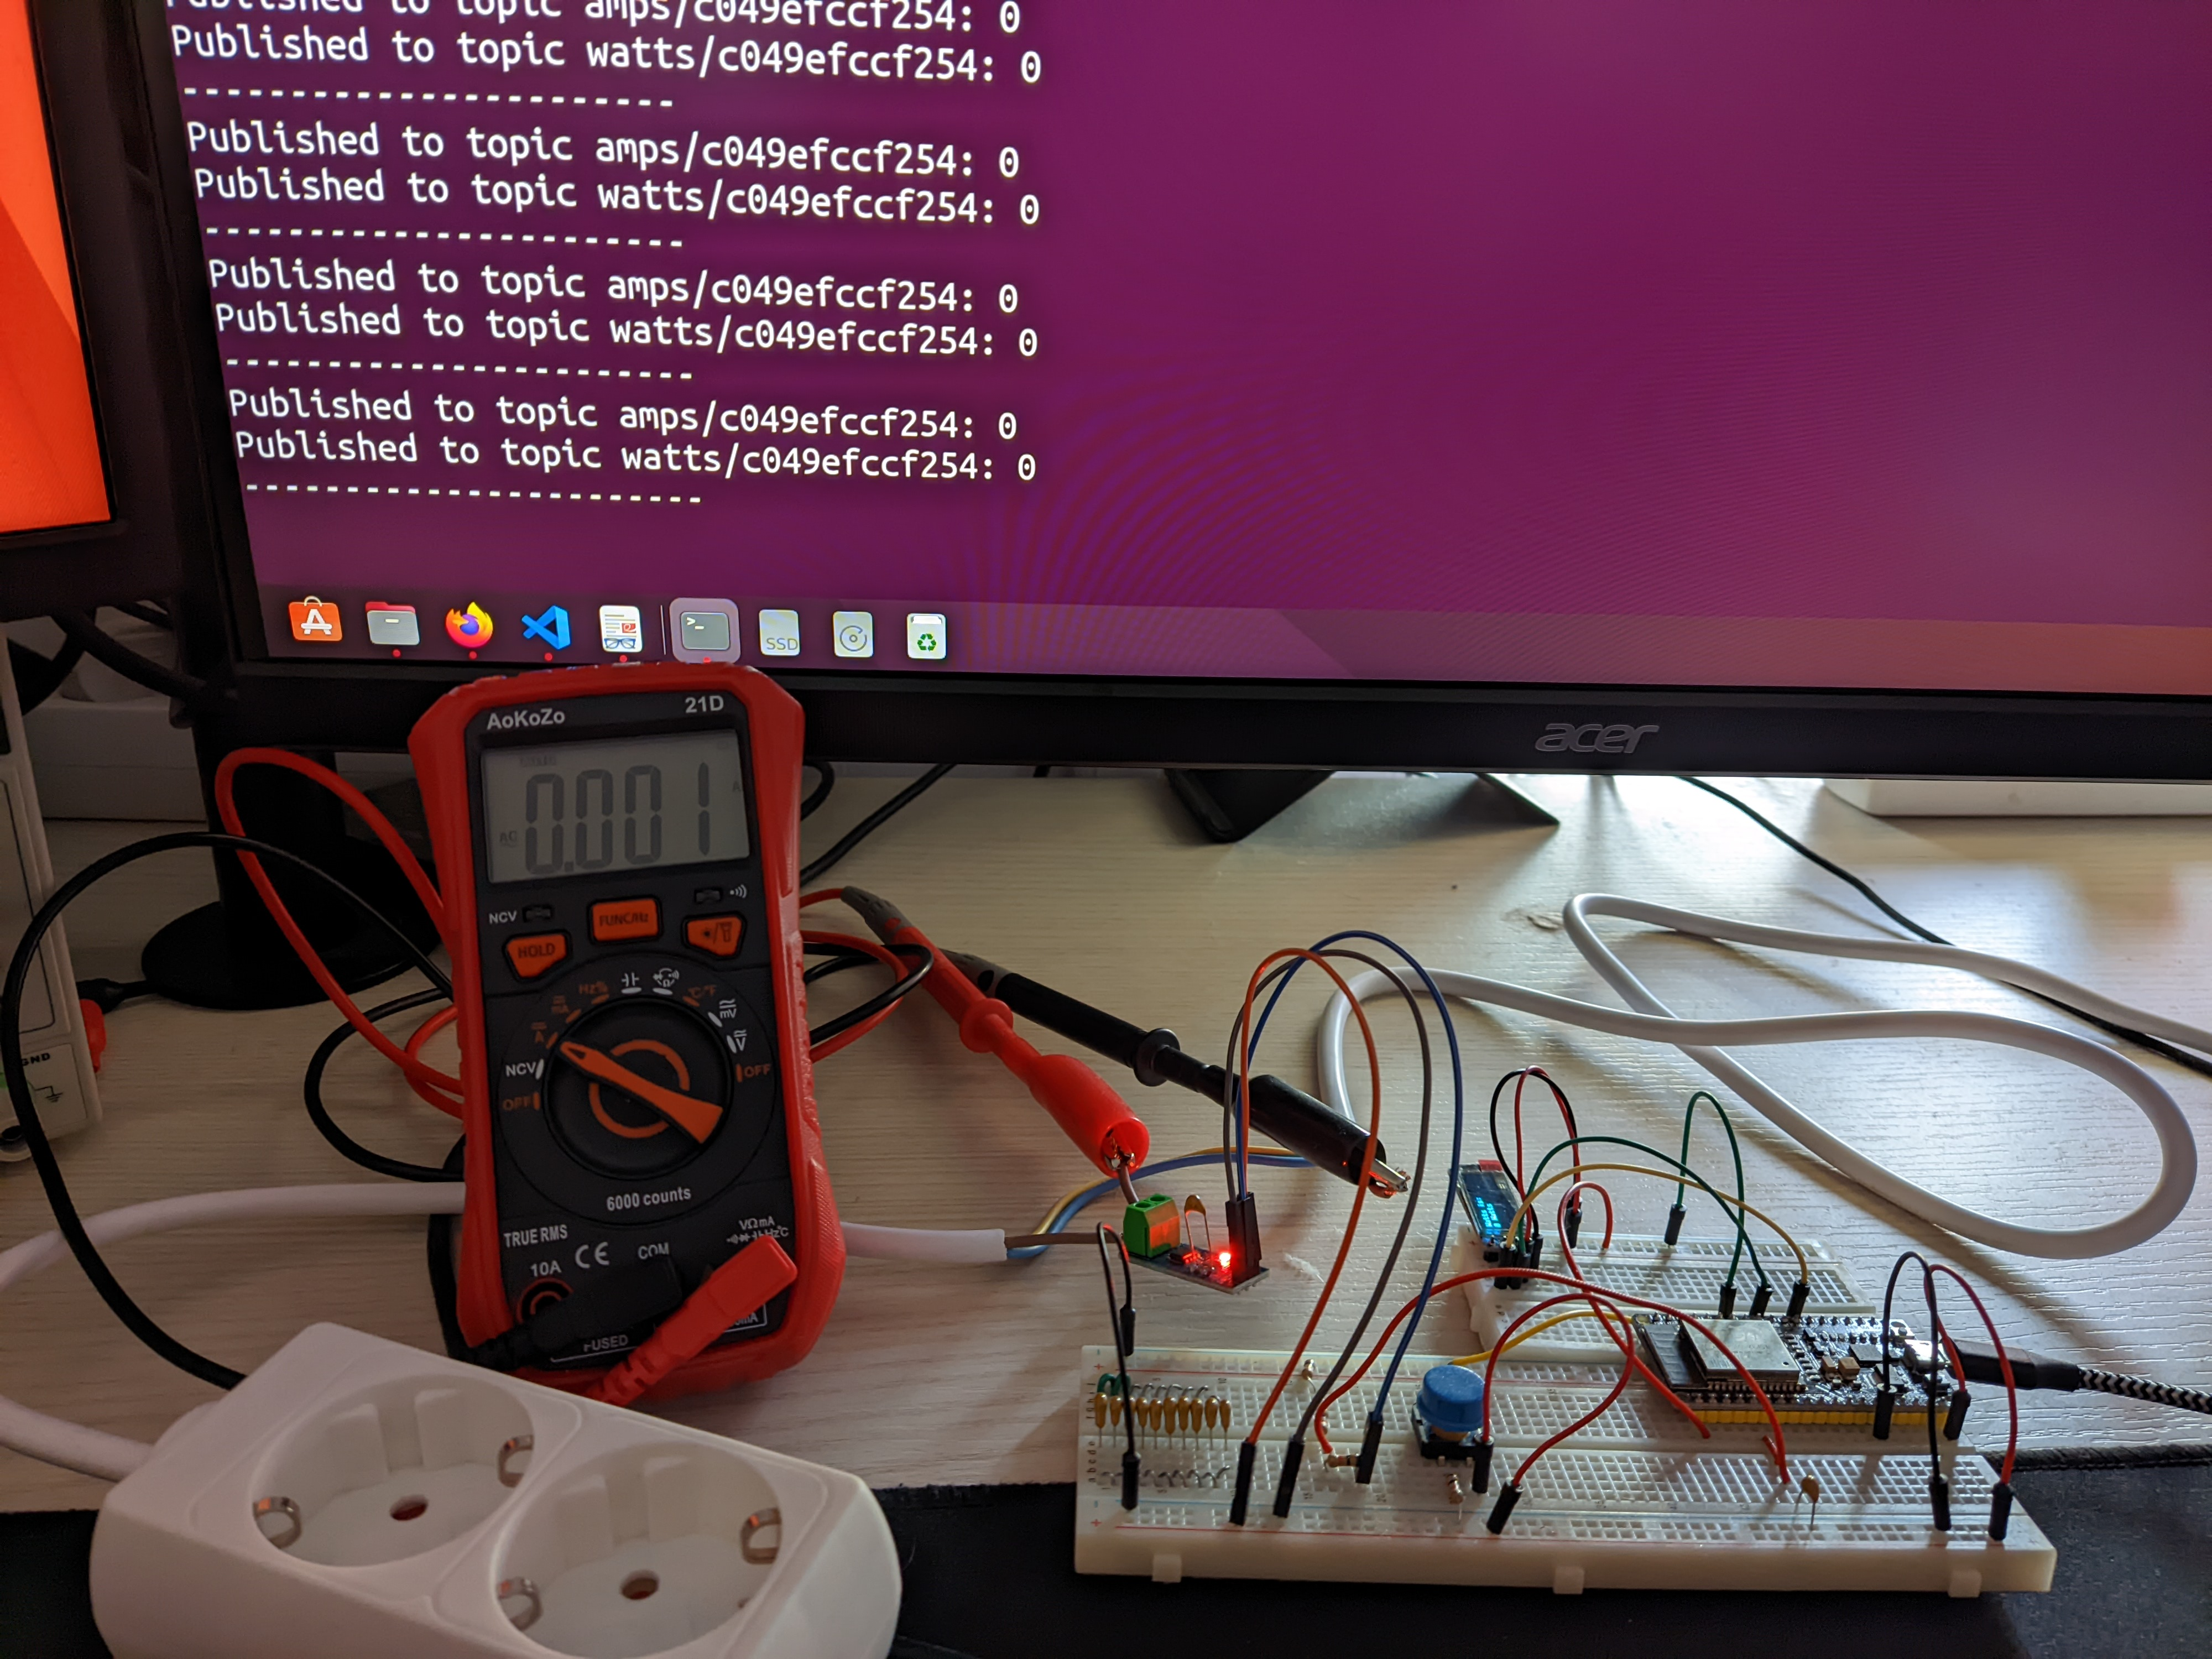
\includegraphics[width=0.5\textwidth]{imagenes/AC_noload.jpg}
	\caption{Nada conectado al enchufe}
\end{figure}
Como podemos observar, ACS712 nos da un valor de 0A al igual que el amperimetro.

\subsubsection{Secador aire frío}
La primera prueba con baja corriente se ha puesto un secador de pelo con la función de solo aire frio. Como solo esta funcionando el motor del secador, podemos observar como hay mas diferencia entre lo que mide el ACS712 y el amperimetro. \\
\begin{figure}[h!]
	\centering
	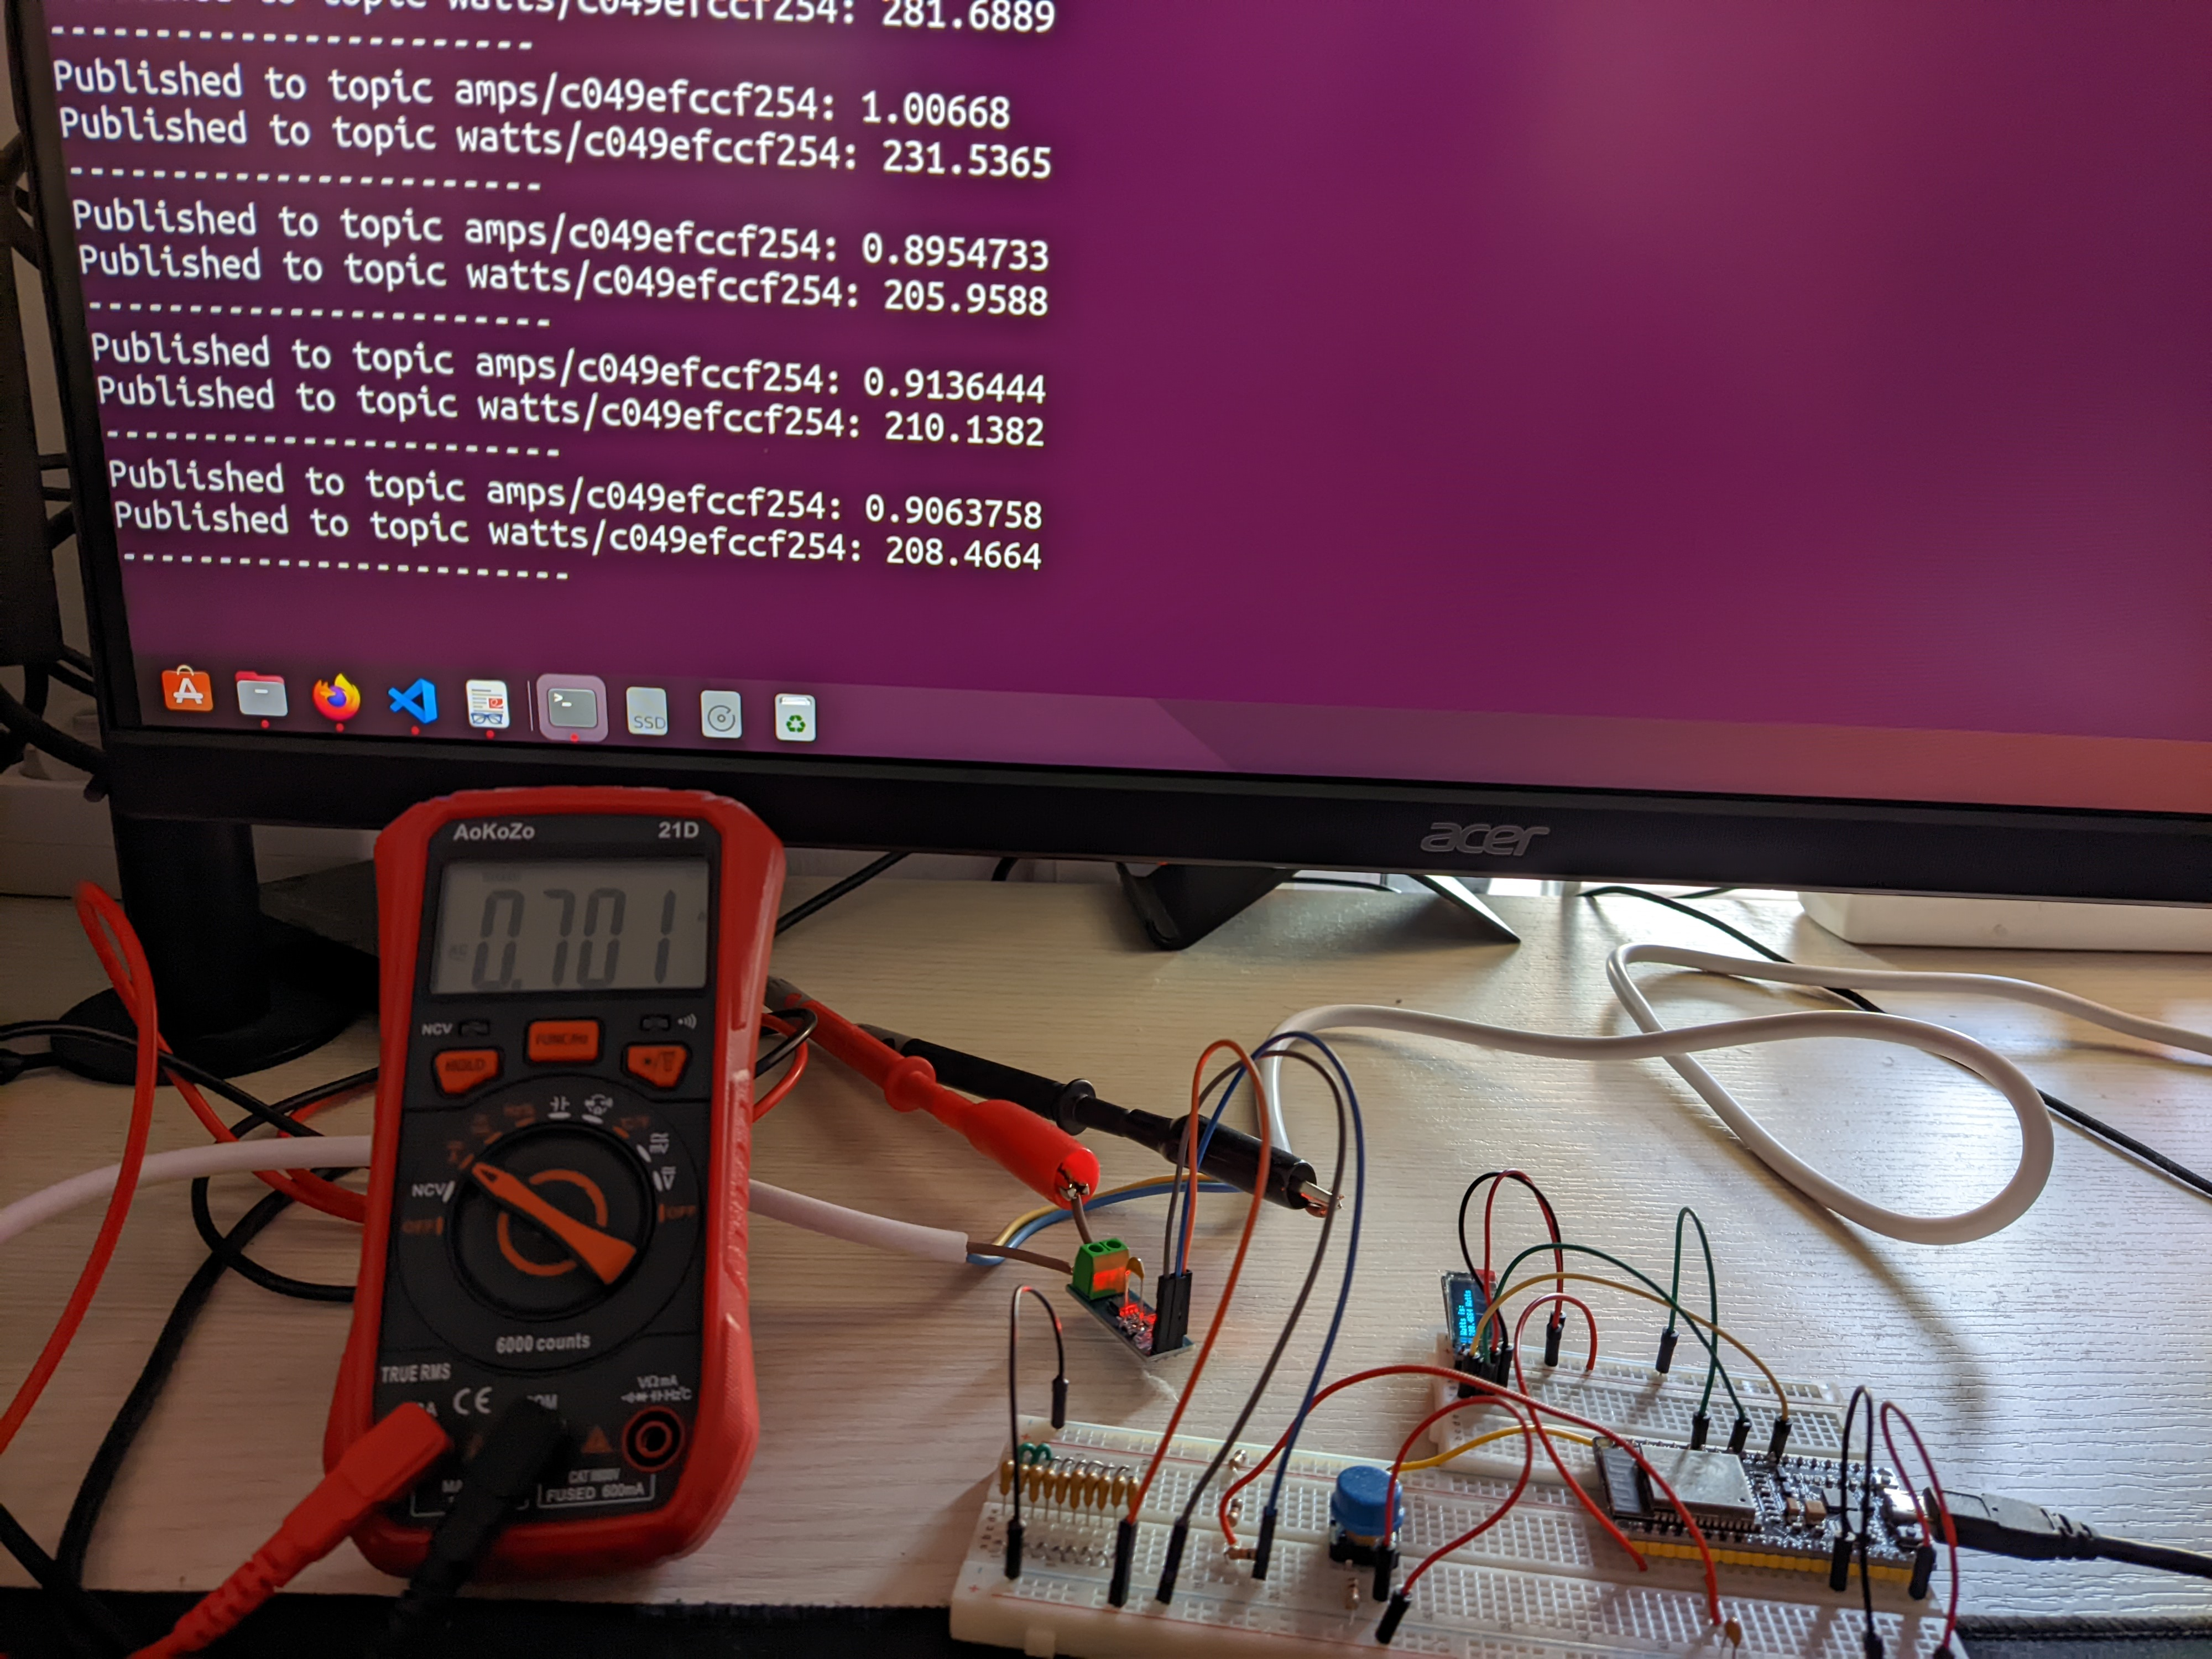
\includegraphics[width=0.5\textwidth]{imagenes/AC_O_7Amps.jpg}
	\caption{Secador de pelo solo con la función de aire frio}
\end{figure}
El amperimetro mide 0.701A y el ACS712 0.961A. \\

\subsubsection{Secador aire caliente al minimo}
La siguiente prueba la hacemos con el secador de pelo con la función de aire caliente pero a nivel bajo de calor.\\
\begin{figure}[h!]
	\centering
	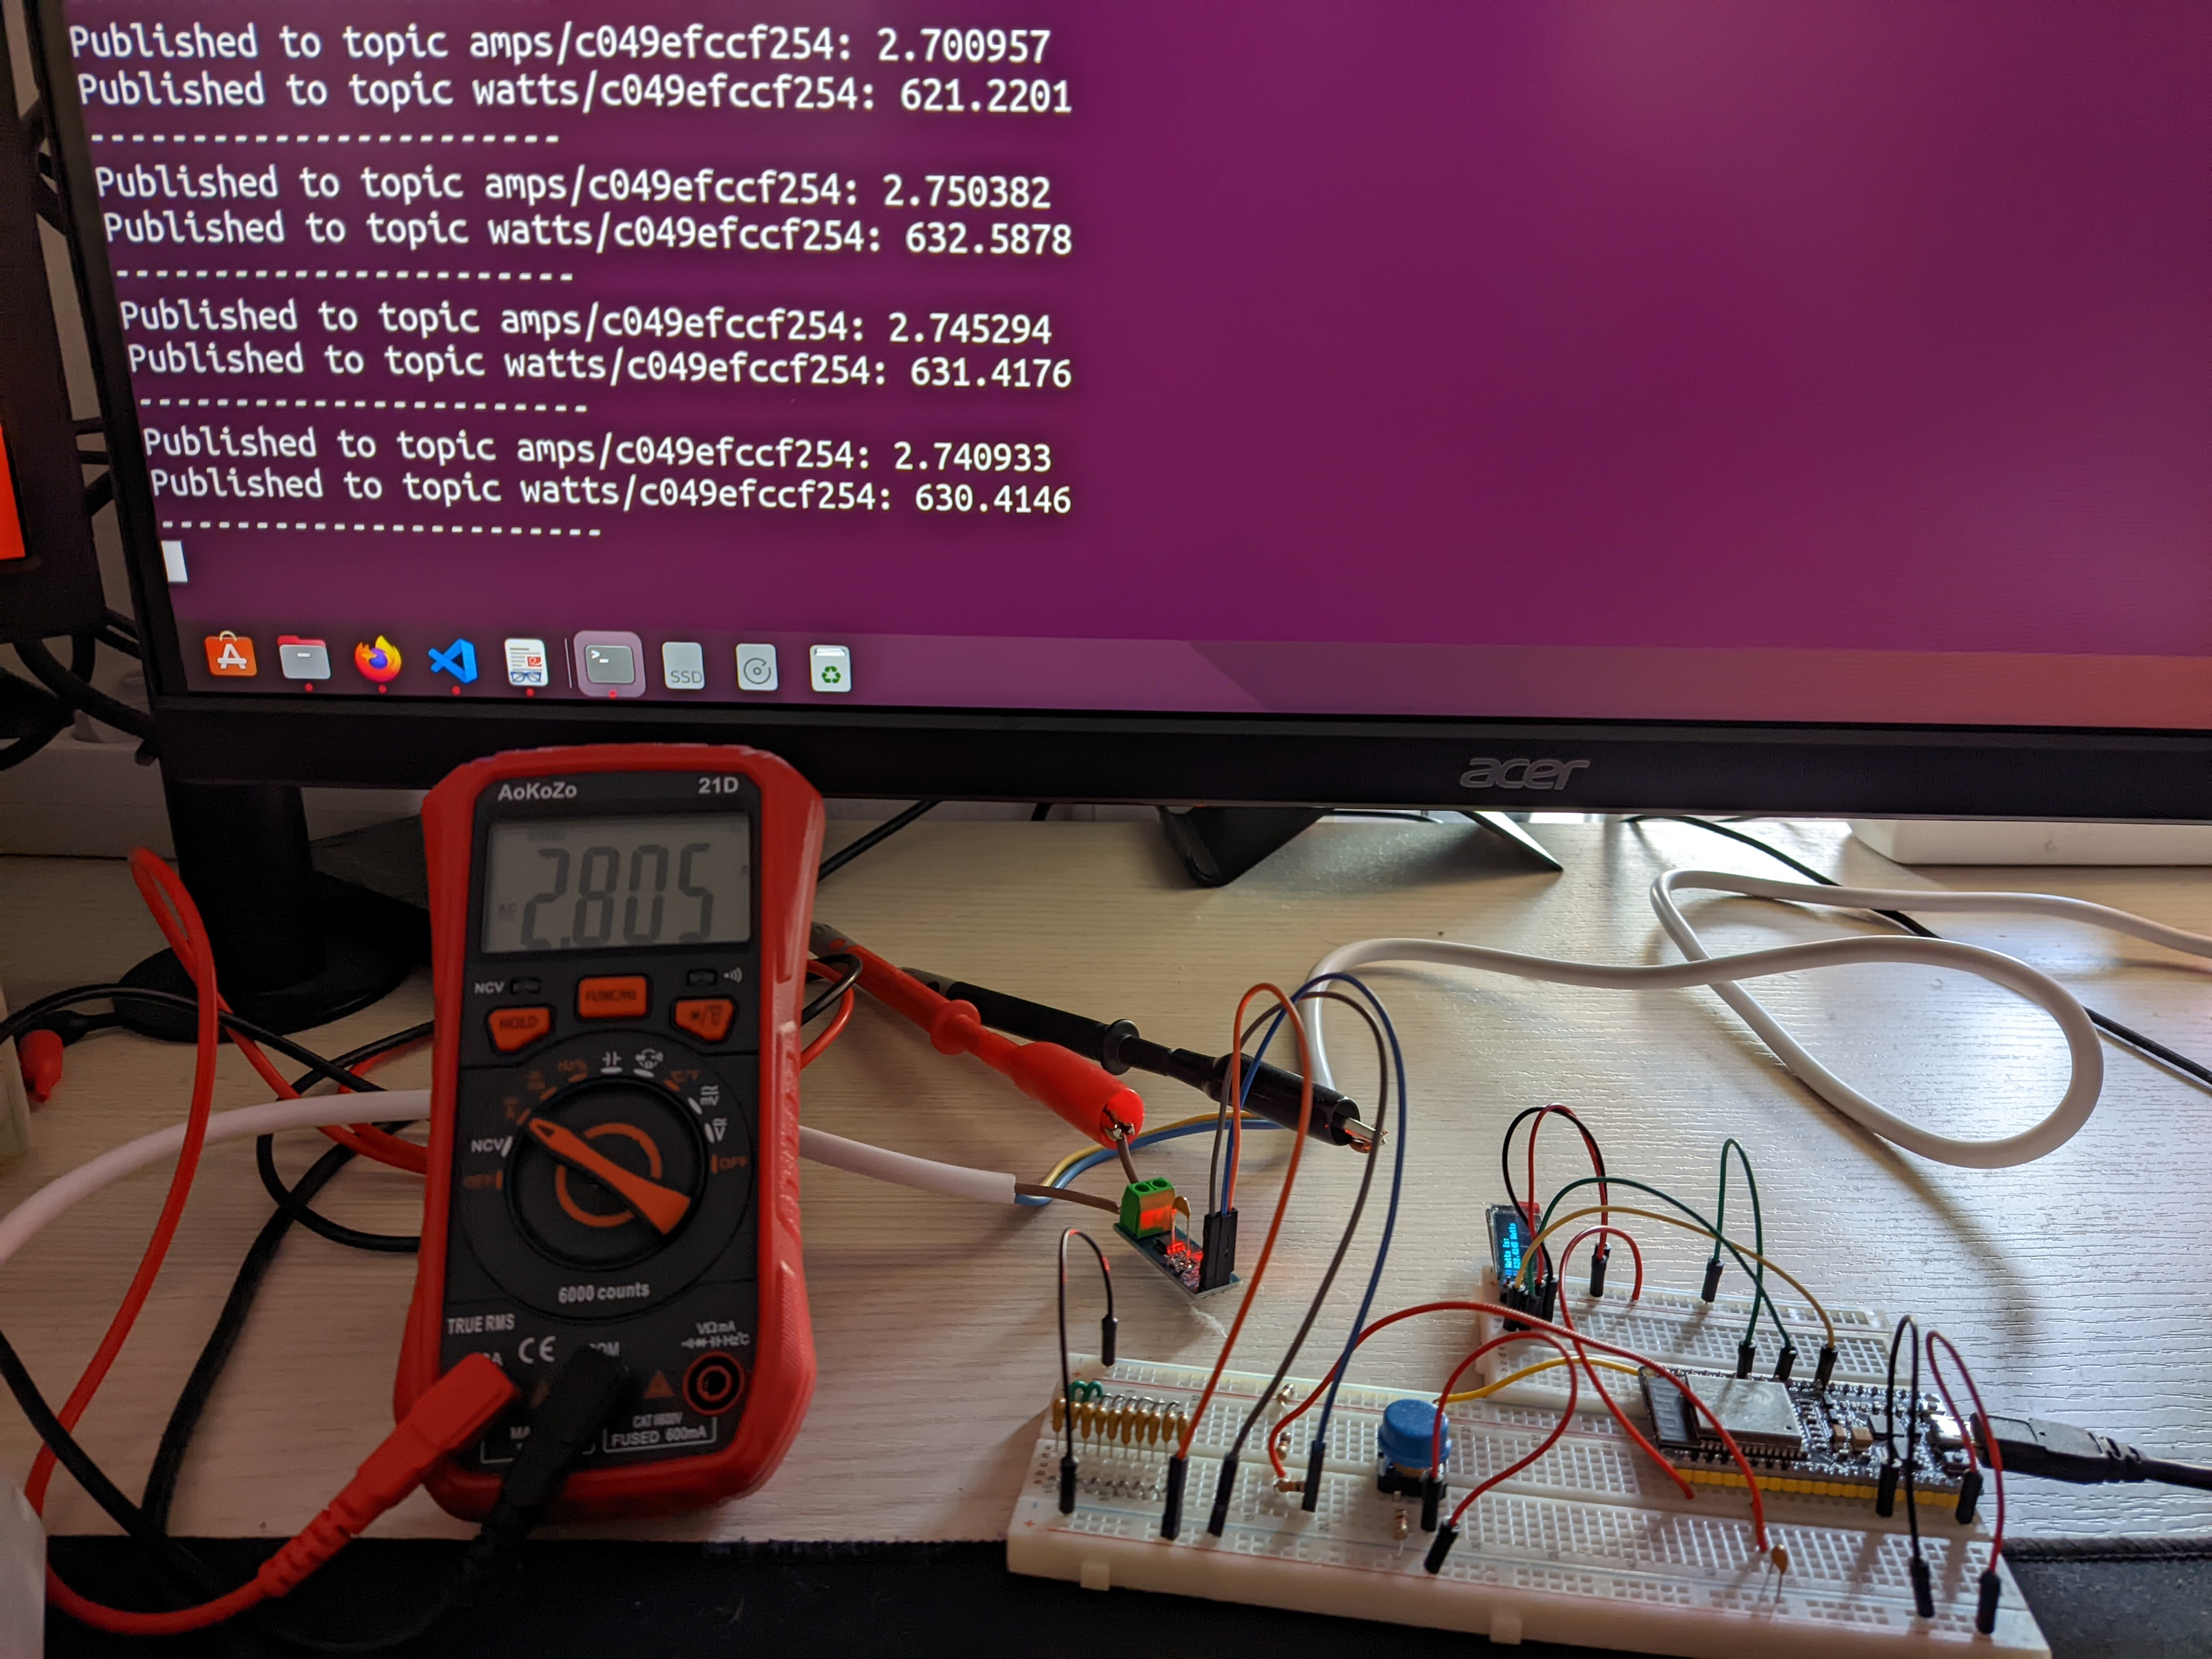
\includegraphics[width=0.5\textwidth]{imagenes/AC_2_8Amps.jpg}
	\caption{Secador de pelo solo con la función de aire caliente a nivel bajo de calor.}
\end{figure}
Al estar usando el secador las resistencias para generar aire caliente, podemos observar como aqui si que medimos con el ACS712 casi igual que con el amperimetro.
El amperimetro mide 2.8A y el ACS712 2.75A. \\
\subsubsection{Secador aire caliente al máximo}
La última prueba la hacemos con el secador de pelo con la función de aire caliente al máximo nivel de calor.\\
\begin{figure}[h!]
	\centering
	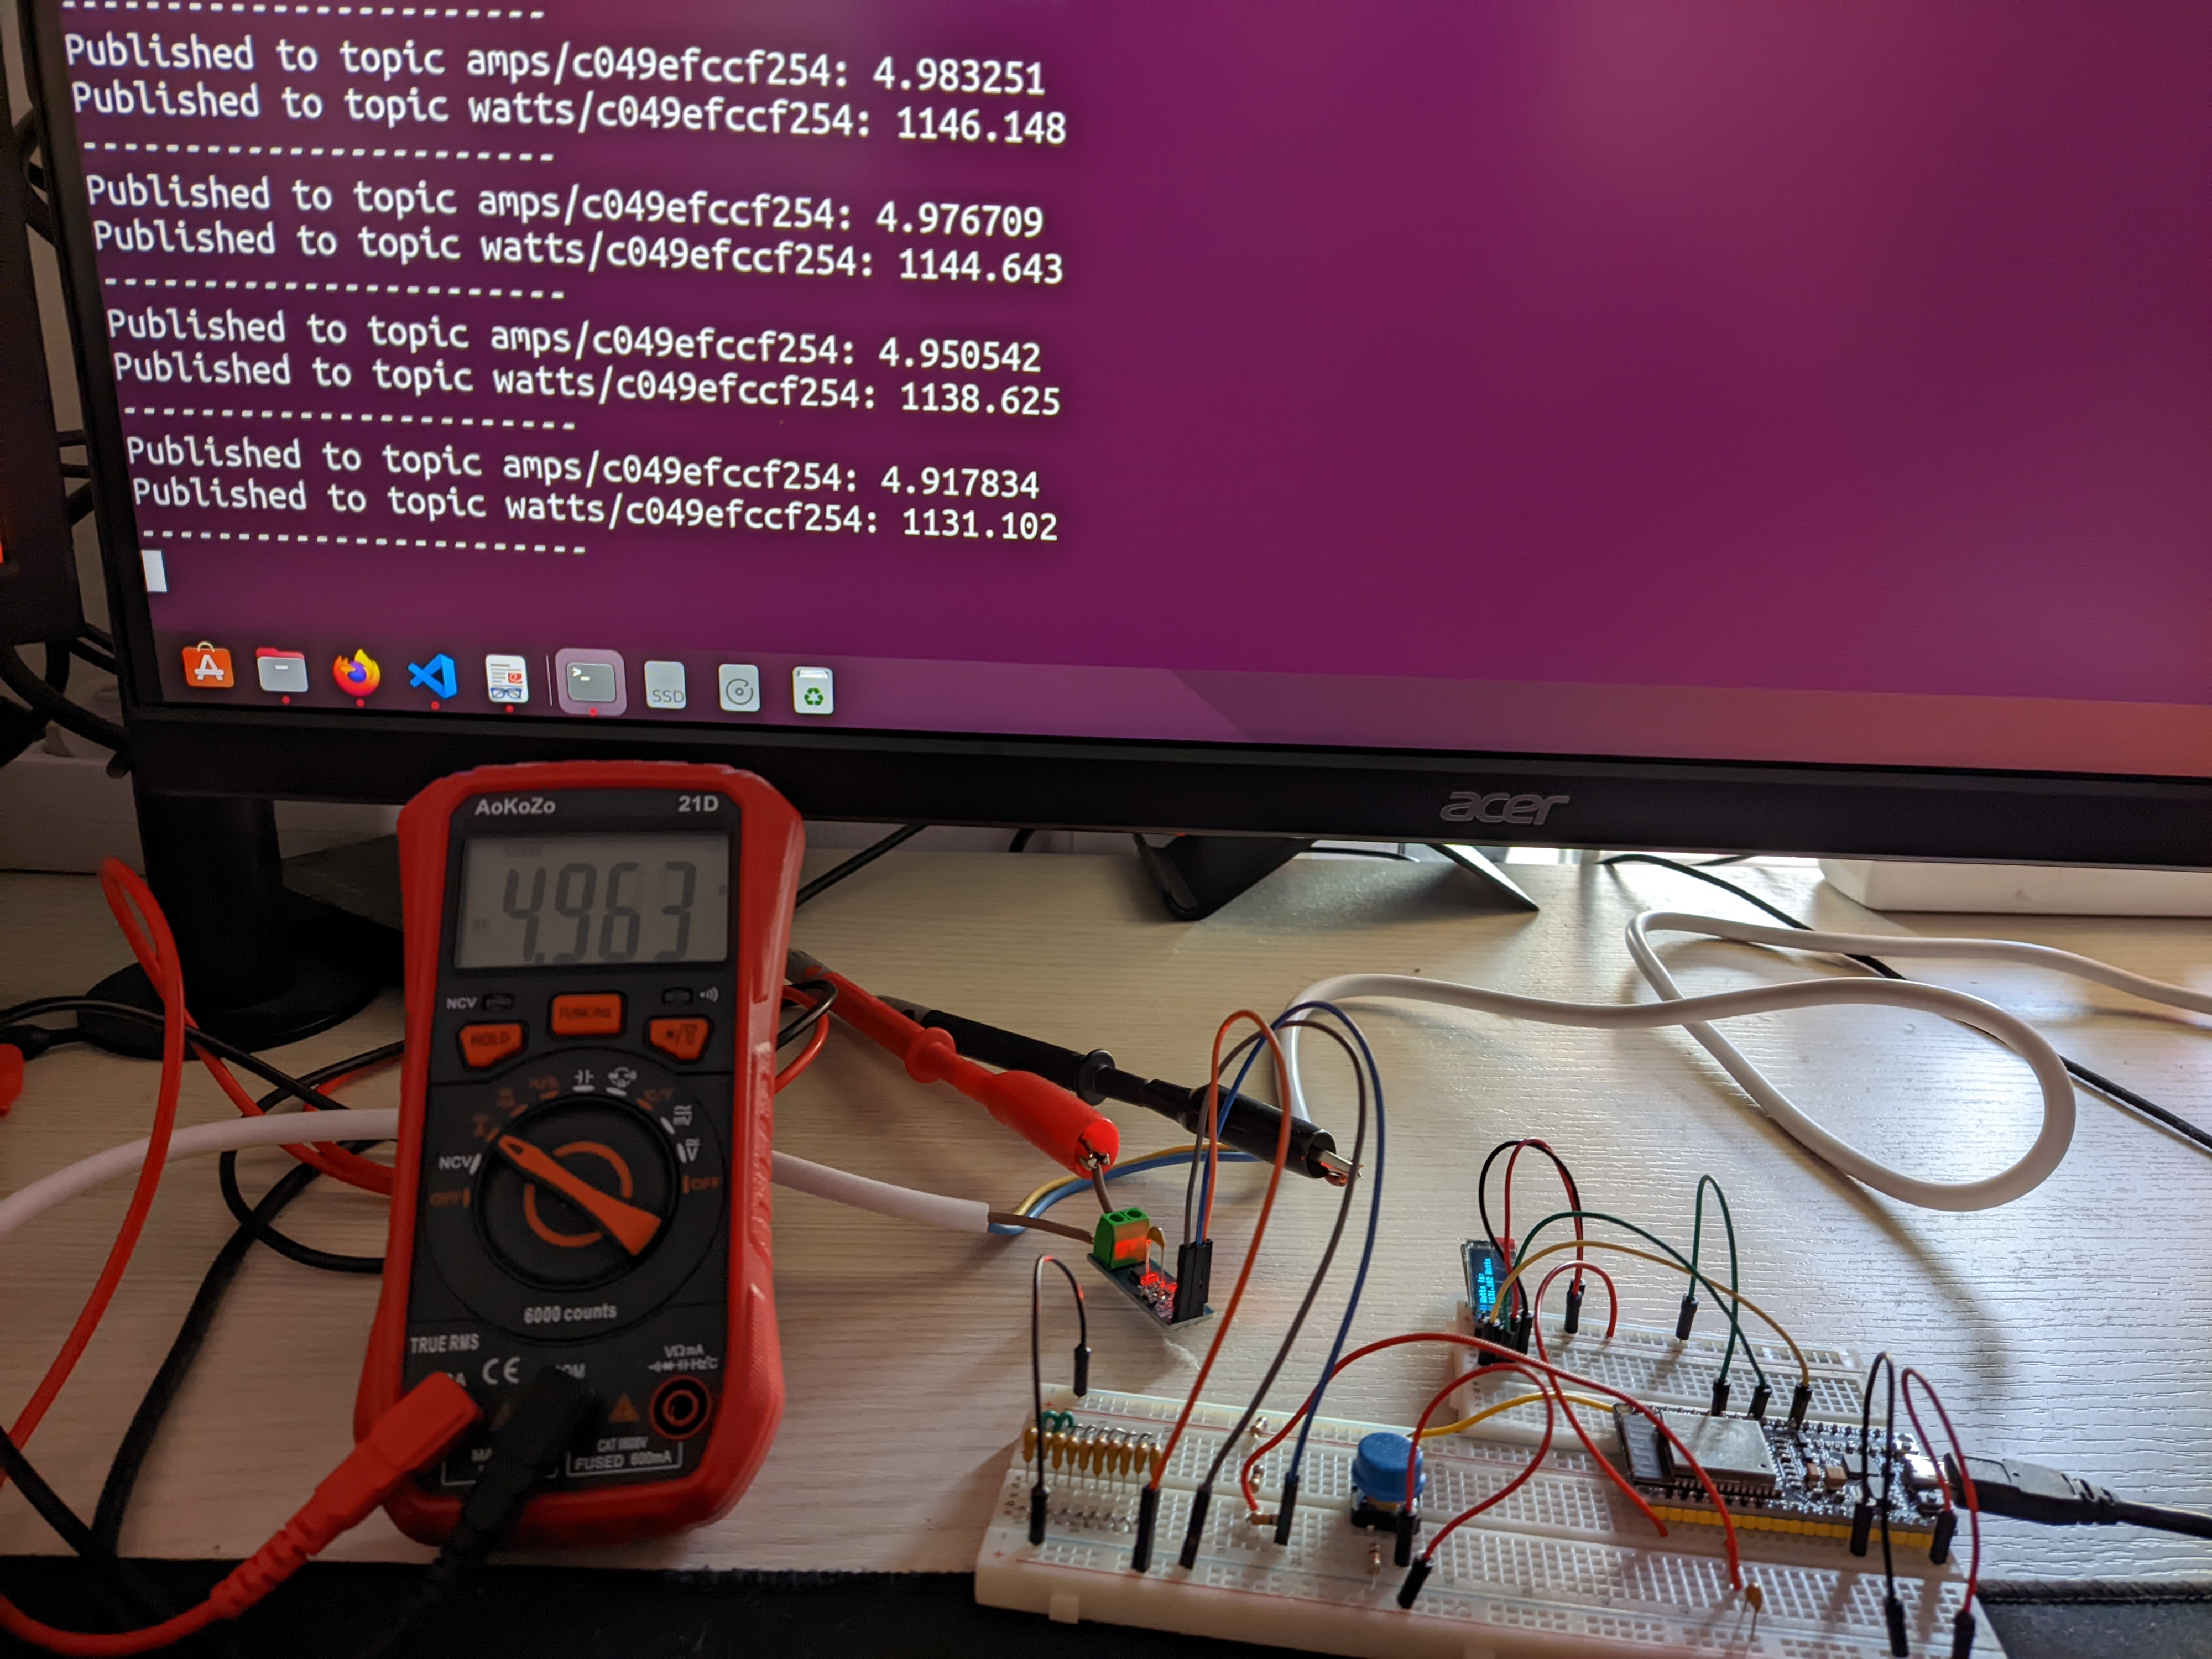
\includegraphics[width=0.5\textwidth]{imagenes/AC_4_9Amps.jpg}
	\caption{Secador de pelo solo con la función de aire caliente a nivel máximo de calor.}
\end{figure}
El ACS712 podemos observar como mide 4.95A y el amperimetro 4.963A.\\

\subsection{Sensor de voltaje}
Al no disponer de una fuente de alimentación que genere voltaje alterno, lo que voy a probar es el sensor en diferentes redes electricas (en diferentes casas). \\
\subsubsection{Casa 1}

INSERTAR IMAGEN SENSOR DE VOLTAJE CON MULTIMETRO ENSEÑANDO TMB EL VOLTAJE
\subsubsection{Casa 2}

\subsubsection{Casa 3}

\subsubsection{Casa 4}


\newpage
\end{titlepage}
